\chapter{Credit Assignment in the Brain}

\subsection{Introduction}

In this chapter we shift gears again and now consider applications of the free energy principle to the problems of \emph{learning} in the brain. Specifically, here we aim to understand the nature of credit assignment in the brain, and focus on how and whether the backpropagation of error algorithm which underpins all the recent successes of machine learning in training deep artificial neural networks, could potentially be implemented in the brain. In this chapter, we present the fruit of our work investigating this extremely important question for the case of rate-coded integrate and fire neurons engaged in a static task (such as object recognition), where there is only a feedforward pass to be concerned with and all backpropagation is through space, and not time. While this setting is considerably simplified from the one the brain faces in reality, it is also much more tractable and well-understood and solving the problem in this domain may provide vital clues into the full solution. 

This chapter is split into four relatively independent sections. In the first section, we provide a general introduction and mini literature review on backpropagation and previous attempts to derive biologically plausible algorithms to implement backpropagation in the brain.  In the next two sections, we  then present our work deriving new algorithms for biologically plausible approximations to the backpropagation of error algorithm. 

In the first section, we show that predictive coding -- the free energy process theory from chapter 3 -- can, if setup correctly, exactly approximate the backproapgation of error algorithm along arbitrary computation graphs. This result is fascinating since predictive coding has a long history and well-developed literature on its properties, performance, and especially its biological plausibility, as well as possessing several well-developed theoretical neural implementations \citep{bastos2012canonical,keller2018predictive,kanai2015cerebral}. We empirically validate this approximation to backprop and showcase that predictive coding can perform equally to backprop at training complex machine learning architectures such as CNNs and LSTMs. 

Secondly, we develop a novel algorithm -- \emph{Activation Relaxation} (AR) -- which also can asymptotically converge to the required backpropagation error gradients using only local connectivity -- and which does not require two separate population of value and error neurons. We empirically show that this algorithm can train complex machine learning architectures with performance equal to backprop and, additionally, demonstrate that the same relaxations shown in Chapter 3 for predictive coding -- such as using learnable backwards weights to overcome the weight transport problem, and dropping the nonlinear derivatives also work for the AR algorithm, thus importantly both substantially improving the overall biological plausibility of the AR algorithm as well as demonstrating the generalizability of the results in Chapter 3 to other algorithms.

Finally, in the third section, we have included a more speculative discussion on a potential further algorithm for solving backprop in rate-coded neurons directly, instead of in an iterative fashion. We discuss the possible limitations of this algorithm as well as the required neural circuitry and, for the first time, begin to precisely understand what the key problems are for the rate-coded sense and also what a real solution would look like.

\subsection{Backpropagation in the Brain}

Due to the immense success of machine learning approaches based upon connectionist deep neural networks trained upon the backpropagation of error algorithm, our paradigms on how the brain functions is also shifting. Specifically, the paradigm that the brain, or at least the neocortex, is fundamentally a blank-slate learning machine which uses general purpose learning algorithms to handle inputs, akin to a deep neural network is becoming increasingly influential in neuroscience, partially displacing older views that the brain consists of a series of separate `modules' \citep{fodor1983modularity,pinker2003language}, each of which performs a single specialized function using what are effectively specific and pre-set algorithms, hard-coded over the course of evolutionary history. While functional specialisation is an extremely notable characteristic of the brain, it is more widely believed that this specialisation, especially in the cortex, is due to differences in input and small inductive biases shaping the nature and output of a very general learning algorithm which is implemented throughout the cortex, rather than each functional module possessing its own independent and isolated suite of algorithms. This view is supported by evidence of a remarkable uniformity of cortical cytoarchitecture and neuroanatomy, belied by the heterogeneity observed in subcortical areas \citep{bear2020neuroscience}.

While, for a long time, it was empirically unclear whether the fundamentals of intelligence -- such as robust and generalizable perception, natural language capabilities, and adaptive action planning -- could emerge solely from learning algorithms with relatively few inductive biases, applied to vast amounts of data, the past decade and its immense advances in machine learning have proven precisely this. Modern machine learning, effectively, represents the culmination and empirical verification of earlier connectionist theory \citep{rumelhart1986learning}.

This view places the central focus on learning. Since the backpropagation of error algorithm has proven so immensely successful in machine learning, to train an extremely wide variety of architectures to perform an impressive array of tasks \citep{krizhevsky2012imagenet,goodfellow2014generative,radford2019language,schrittwieser2019mastering,schmidhuber1999artificial}, and given that the brain itself faces an almost identical credit assignment problem in having to adjust synaptic strengths to allow for learning to occur, it is a very interesting and important question to ask whether learning algorithm implemented in the brain could simply be backprop. If this question were conclusively answered in the affirmative, it would represent an enormous conceptual breakthrough in neuroscience since it would provide, for the first time, a general and powerful organizing principle for the brain (or at least the cortex) as a whole, it would allow the importation directly into neuroscience of a large quantity of results from machine learning. Such an answer would additionally have deep philosophical implications. It would imply that there is very little effective difference between current machine learning methods and the kinds of learning, inference, and planning algorithms that are implemented in the brain to give rise to undeniably intelligent and apparently conscious behaviour, and as such would imply that the current paradigm in machine learning suffices, with more scale and potentially more expressive architectures, to create fully general intelligences akin to humans or beyond \citep{bostrom2017superintelligence}.

On the other hand, if it were shown that the brain were conclusively not doing backprop, then this would also be an advance, although a lesser one, in neuroscience. Such a conclusion would necessarily shed light upon the actual algorithms utilized by the brain for credit assignment and learning, which would provide both a general principle for understanding the function and operation of the brain over time, as well as undoubtedly provide key insights for machine learning in developing, improving, and scaling up current methods. 

The theory and algorithm for backpropagation of error (Backprop) emerges in the 1970s \citep{linnainmaa1970representation}, and by the 1980s was widely used for training connectionist neural networks \citep{rumelhart1985feature,rumelhart1986learning,griewank1989automatic} Already in the 1980s, researchers had proposed that backprop could be implemented in the brain, and tried to find commonalities between then contemporary neuroscience and progress in connectionist modelling using neural networks \citep{rumelhart1986learning}. However, a number of articles argued convincingly that a direct implementation of backpropagation is biologically implausible \citep{crick1989recent}, which dampened down potential interest in this connection considerably until the question was re-raised by the successes of machine learning in the 2010s. Before investigating the ways in which backpropagation appears biologically implausible, and how these issues might be addressed, we first give a detailed introduction to the backprop algorithm.

First we must decide on some terminology. Neural networks are typically trained to minimize some loss function $\mathcal{L}$. 
The credit assignment problem concerns the \emph{computation of the derivatives} of the loss with respect to every parameter of the network $\frac{\partial \mathcal{L}}{\partial W}$. Backpropagation of error is an algorithm that solves the credit assignment problem exactly using the technique of \emph{Automatic Differentiation} (AD) \citep{griewank1989automatic,baydin2017automatic,van2018automatic,paszke2017automatic}. \footnote{There are other methods for computing derivatives, such as finite differences, but they are less accurate and more computationally costly than AD and are not generally used in machine learning} . Given these derivatives, the network can be trained with the stochastic gradient descent algorithm $W_{t+1} = W_t + \eta \frac{\partial \mathcal{L}}{\partial W}$. However, given the gradients computed by backprop, other gradient algorithms are possible including a variety of modified descent procedures such as Nesterov Momentum \citep{nesterov27method}, RMS-prop \citep{hinton2012neural} and Adam \citep{kingma2014adam} second order methods such as natural gradients \citep{amari1995information} and Gauss-Newton optimization, as well as stochastic sampling methods such as stochastic langevin dynamics \citep{welling2011bayesian}, and Hamiltonian MCMC \citep{neal2011mcmc}.

The fundamental mathematics underlying backprop is the chain rule of calculus. Essentially, if we have a function -- such as a neural network -- which consists of the composition of many differentiable functions, then we can express the derivative of large function as a product of the derivatives of all the component functions with respect to one another. Suppose we have the forward function and loss function,
\begin{align*}
&\hat{y} = f^L(W^L f^{L-1}(W^{l-1} f^{L-2}(\dots f^0(W^0 x)))) \\
& \mathcal{L} = g(\hat{y}, t) \numberthis
\end{align*}
where $\hat{y}$ is the prediction outputted by the neural network, $L$ is the number of layers, $[f^L \dots f^0]$ is the activation functions for each layer and $[W^L \dots W^0]$ is the weights or parameters for each layer. $\mathcal{L}$ is the overall loss function, $t$ is the desired target outputs and $g$ is the loss function. With this forward function, we can compute the derivative of the loss with respect to any parameter set -- for instance $W^0$ using the chain rule,
\begin{align*}
\label{chain_rule_equation}
\frac{\partial \mathcal{L}}{\partial W^0} = \frac{\partial \mathcal{L}}{\partial \hat{y}}\frac{\partial \hat{y}}{\partial y^{L}} \big[ \prod_{l=L}^{l=1} \frac{\partial y^l}{\partial y^{l-1}} \big] \frac{\partial y^1}{\partial W^0} \numberthis
\end{align*}
which allows us to express the derivative of a product of all the derivatives of the intermediate component functions. In general, this is possible for any function as long as every component function is differentiable. We can represent any function as a \emph{computation graph} which is a graph where each intermediate step in the computation is a vertex and each component function is an edge. While this example, and most simple neural network, is simply a chain graph, other more complex graphs are possible. If there are multiple paths through the graph, the derivatives of the paths are summed together. As long as every component function is differentiable, every one of the derivatives in Equation \ref{chain_rule_equation} can be explicitly computed and evaluated, thus allowing the full derivative $\frac{\partial \mathcal{L}}{\partial W^0}$ to be computed explicitly. Importantly, the computational cost of such an evaluation is generally linear in the number of component functions -- and thus is of approximately the same complexity as simply evaluating the function in the first place. AD approaches like this, then, allow for the evaluation of derivatives of any differentiable computation for a low and constant additional computational cost -- allowing for their widespread use within machine learning.

There are two approaches in AD to computing the chain of derivatives as in Equation \ref{chain_rule_equation}, which are called `forward-mode' and `reverse-mode' AD. The difference between these methods is effectively whether the product of derivatives is computed from right to left (forward-mode) or left to right (reverse mode). Forward-mode effectively accumulates the gradients starting with the initial jacobian $\frac{\partial y^1}{\partial W^0}$ and then moving leftwards down the chain, in the same direction as the original function evaluation. This allows derivative evaluation to take place in parallel with original function evaluation through the use of `dual numbers' \citep{griewank1989automatic} which extend every number with an `derivative part' analogous to how complex numbers extend real numbers with a complex part. Since dual-numbers can be evaluated in parallel with the original function evaluation, the computational cost of forward-mode AD is of the order of the input dimension and it has a constant memory cost, since no intermediate products need to be stored in memory.

Reverse-mode AD, conversely, evaluates the chain of derivatives from left to right. That is, it starts with and accumulates onto the vector $\frac{\partial \mathcal{L}}{\partial \hat{y}}$, which is also called the \emph{adjoint} or \emph{pullback} \footnote{In continuous time, Equation \ref{reverse_mode_equation} becomes the adjoint ODE}. It then iterates recursively `backwards' through the chain using the following equation,
\begin{align*}
\label{reverse_mode_equation}
    \frac{\partial \mathcal{L}}{\partial y^l} = \sum_j \frac{\partial \mathcal{L}}{\partial y_j^{l+1}} \frac{\partial y_j^{l+1}}{\partial y^l} \numberthis
\end{align*}
where the sum simply states that if there are multiple potential paths in the graph, they should be summed together. Since it starts at the `end' and works backwards, reverse-mode AD requires the function to be evaluated first after which the derivatives can begin to be computed in a backwards sweep, thus leading reverse-mode AD to use characteristic forward (function evaluation) and backwards (derivative evaluation) sweeps. Since all intermediate activities must be stored in memory, reverse-mode AD has a memory cost linear in the number of component functions, as well as a computational cost which scales with the dimension of the output. Since neural networks typically have a scalar output loss and very high dimensional inputs (such as image pixels), reverse-mode AD is typically computationally cheaper and is the method used in practice for training deep networks. Reverse mode AD also has the advantage that it backpropagates the gradients back to where the weights are directly, while forward-mode AD does compute the weights, but they are all bunched up at the end of the graph by the loss, and therefore would need, in a physical system such as the brain, to be transmitted back to where the weights were originally as well.

Here, we focus primarily on the implementation of reverse-mode AD in the brain due to its generally superior computational capabilities (and avoidance of this weight locality problem for forward mode AD). It is possible, however, that the brain may use some combination of forward and reverse mode in practice. One especially appealing method is to use reverse-mode AD to handle hierarchical networks -- i.e. nonlocality in space, while using forward mode AD to handle recurrent credit assignment through time. Here forward mode AD has the clear advantage that the gradients move forward in time at the same rate as the weights themselves, so that there is no locality problem here. In fact, the locality problem now afflicts reverse-mode AD which, in this circumstance, needs to backpropagate gradients \emph{backwards through time}, which is problematic. Here we do not address the temporal credit assignment problem and focus entirely on backpropagation through space, where we assume reverse-mode AD is the best approach.

Although reverse-mode AD is a well characterised algorithm, it is not at all clear whether it can be implementated in the brain. Specifically, backpropagation has three principal problems which make its apparent biological plausibility dubious -- firstly, backpropagation appears to require non-local information transfer, since the gradient of the synaptic weights depends on activity from the rest of the network which ultimately leads to the final loss outcome. Secondly, if we look at the specific case of a rate-coded standard integrate and fire model, whereby the output is a function of the input and the synaptic weights,
\begin{align*}
    y^{l+1} = f(W^l y^l) \numberthis
\end{align*}
then the derivative of the loss with respect to the pre-activations becomes,
\begin{align*}
    \frac{\partial \mathcal{L}}{\partial y_l} = \frac{\partial \mathcal{L}}{\partial y^{l+1}} \frac{\partial f(W^l y^l)}{\partial y^l} {W^l}^T \numberthis
\end{align*}
which requires both the derivative of the activation function, which may or may not be easy to compute locally, and also the transpose of the feedforward weights ${W^l}^T$. This transpose is problematic since effectively it requires the backwards pass activations to be sent `backwards' through the forwards weights -- a process which is biologically implausible. This problem is called the `weight transport problem'. Finally, if we look at the update rule for the weights themselves,
\begin{align*}
\frac{\partial \mathcal{L}}{\partial W^l} = \frac{\partial \mathcal{L}}{\partial y^{l+1}} \frac{\partial f(W^l y^l)}{\partial W^l} y^L \numberthis
\end{align*}
which while it does depend on the pre-synaptic activations $y^l$ also depends on the adjoint vector $\frac{\partial \mathcal{L}}{\partial y^{l+1}} $ which is generally non-local. Interestingly, the update rule specifically does \emph{not} depend at all on the post-synaptic activity, in contrast to the widely accepted view of Hebbian plasticity being implemented in the brain, although it does depend on the \emph{derivative} of the post-synaptic activity with respect to the weights $\frac{\partial f(W^l y^l)}{\partial W^l}$, which may or may not be difficult to compute. The issue first of computing the adjoint vector $\frac{\partial \mathcal{L}}{\partial y^{l+1}}$ in a biologically plausible manner, and then transmitting it to the required synapses, since it is non-local, thus form the core issue standing in the way of any biologically plausible implementation of reverse-mode AD. A final issue relates to the need, in reverse-mode AD, for separate forward and backwards phases, while the brain presumably needs to operate continuously in time. It has been suggested that the brain's rhythmic oscillations \citep{buzsaki2006rhythms} may allow it to `multiplex' forward and backward passes together, although this intuition has not yet, to my knowledge, been made precise in the literature.

Due to a general understanding that backpropagation is biologically implausible, much research has focused on other potentially more biologically plausible methods by which the brain might learn. A large amount of attention has focused on Hebbian update rules \citep{gerstner2002mathematical}, which only utilize the post and pre synaptic activities, based on the initial intuitions of Donald Hebb \citep{hebb1949first}. A number of variants of Hebbian learning have been proposed, and the full class of potential algorithms has been exhaustively analysed in \citep{baldi2016theory}. However, a key issue with Hebbian learning is that, since it can only use local information in the form pre and post synaptic activities, it cannot incorporate information about the distant loss function, and thus allow for the precise goal-directed learning that backprop is capable of. In effect, Hebbian learning can only capture and strengthen the local correlations of firing rates across a network and thus, while it can often be used to solve tasks in shallow networks with just a single or a few hidden layers, it fails to scale successfully to deep layers \citep{lillicrap2019backpropagation}.

A second approach is to use global neuromodulators as a part of a `three-factor' learning rule which includes contributions from both the pre-synaptic and post-synaptic activity as well as this `third-factor' \citep{gershman2018uncertainty} which is often conceptualised to be dopamine, in light of the fact that dopaminergic connections from the mid-brain are well-known to innervate large parts of the cortex \citep{daw2006cortical}. These dopaminergic neurons could be signalling some kind of global reward signal, inducing all neurons to increase their weight when a positive reward is encountered and decrease it when a negative reward occurs \citep{seung2003learning,roelfsema2005attention,lillicrap2020backpropagation}, in a procedure which is effectively equivalent to policy gradient methods from reinforcement learning \citep{williams1989experimental}. While such approaches can, asymptotically, learn complex functions in deep neural networks, their key limitation is that the gradient estimates they compute have extremely high variance, since the global neuromodulator cannot distinguish whether a \emph{particular} weight helped give rise to a reward or not, and thus cannot provide precise feedback like backprop. Instead it takes a substantial amount of trials for the random noise provided by the contributions of all the other neurons in the brain to be averaged out to get at the contribution of just a single synaptic weight, which leads to slow and unstable learning in complex tasks with deep networks \citep{lillicrap2019backpropagation}. Additionally, this approach implicitly assumes that the entire brain is optimized end-to-end for reward, however this seems potentially unlikely given that large parts of the cortices deal with aspects like sensory stimuli which are distant from reward and most likely use auxiliary losses such as their own immediate prediction errors.  Nevertheless, if it turns out that backpropagation is not, in fact, used in the brain, then global neuromodulatory rules like this may be the second best option. Importantly, even if it is the case that the brain does backprop, it likely \emph{also} uses this global neuromodulatory approach in a modulatory function to bias learning towards high reward contingencies and perhaps also to adaptively tune learning rates throughout the cortex so that highly valenced experiences (either positive or negative) have a strong effect on plasticity throughout the brain.

Finally, there is also a small but growing literature attempting to understand how and whether backpropagation can be directly implemented in the brain -- namely whether it is possible to design neural circuits to work around the key limitations proposed earlier. An important line of work tackles the weight transport problem. \citet{lillicrap2016random} demonstrate that in reality precise copying of the forward and backwards weights is not necessary, and in fact random fixed backward weights suffice due to the phenomenon of `feedback alignment' whereby the random feedback weights effectively force the forward weights to align with the backward ones to be able to learn. This approach can be improved by ensuring that the sign of the elements of the feedback weight matrix matches the sign of the forward weight matrix (potentially a more biologically plausible constraint than exact copying of values) \citep{liao2016important}, or else learning the backwards weights using an additional plasticity rule \citep{amit2019deep,akrout2019deep,millidge2020relaxing}. While the feedback alignment technique does not typically scale to deep architectures, as the feedback path becomes increasingly corrupted \citep{bartunov2018assessing}, an approach called direct feedback alignment (DFA) \citep{nokland2016direct}, whereby all layers are directly connected to the output layer through random backwards weights, has been shown to be able to scale to large deep architectures \citep{launay2019principled}, although not the usual convolutional neural networks used in vision. While an impressive result, DFA itself violates known neural connectivity constraints which feature reciprocal connectivity between regions and not every layer receiving direct backwards connections from the `output'. 

Secondly, another line of work has focused on the algorithm of target-propagation \citep{bengio2015early,lee2015difference} which is similar to backprop except that instead of providing gradients back to the weights at each layer it provides targets which can then be optimized locally. These targets are produced by mapping backwards the output of the network `nudged' towards the true target through an inverse mapping at each layer. The intuition, is that we want to find the targets which, if the lower layers had matched their activations, would have produced a final output closer to the target. The past year has seen substantial advances in the theoretical analysis of target-prop, where it is now recognised to not approximate backprop, but instead be performing a hybrid form of Gauss-Newton optimization \citep{bengio2020deriving,meulemans2020theoretical}. While promising, large-scale studies on the stability and scalability of target-prop learning have not yet been done, although initial results are promising \citep{bartunov2018assessing}. Additionally, target-prop does not provide solutions to the weight transport problems (now complicated by the additional necessity of learning the backwards inverse weights), and the necessity of storing and comparing the forward and backward information across phases. The intuition of using the final loss function to compute layer-wise targets has also been applied, with variations, in other works \citep{ororbia2019biologically,ororbia2017learning,kaiser2020synaptic}.

Another approach is to use only local information at the synapses, but use a backwards phase which instead of being purely sequential is treated as a dynamical systems which undergoes multiple iterations. Using this approach, while it takes longer than a sequential backwards pass, also allows using only local information, since the information about the loss can be `leaked' slowly backwards using the dynamics over time instead of having to be explicitly transmitted backwards. This allows the brain to operate using the same dynamical rules at all times, in general, instead of sequential forwards and backwards transmission of information. One key example of such a framework is the algorithm of Equilibrium Propagation \citep{bengio2017stdp,scellier2017equilibrium,scellier2018extending,scellier2018generalization}, which uses two dynamical phases -- a \emph{free phase} where the dynamics of the system are allowed to evolve without any influence of the targets, and a \emph{clamped phase} in which the output units are held at a value nudged towards the targets, which destabilizes the free-phase equilibrium and instead sends the network towards a different clamped equilibrium state. It turns out that the difference between these two states corresponds closely to the gradients which would otherwise have been backpropagated through the network and can thus be used to adjust the synaptic weights \citep{scellier2017equilibrium}. Equilibrium propagation has been extensively tested on small datasets like MNIST and CIFAR, although it is not yet known how well the method scales. Additional problems with EP are its necessary use of two distinct backwards phases and, crucially, the storage of information (the equilibrium in the free-phase, throughout the entirety of the clamped phase before their subtraction to obtain the gradients. Another iterative algorithm which has been shown to approximate backprop is predictive coding \citep{whittington2017approximation}.

In this thesis chapter, we make two contributions to the theory of iterative algorithms for approximating backprop. Firstly, we extend work by \citet{whittington2017approximation}, showing that predictive coding can approximate backprop by making this claim precise and exact, and extending it to arbitrary computation graphs \citep{millidge2020predictive}. Specifically, we show that predictive coding provides a fully general iterative approach to approximating reverse-mode automatic differentiation through an identification of the equilibrium prediction error with the adjoint term. This allows us to define predictive coding networks which can train any contemporary machine learning architecture with accuracy equivalent to backprop in a local and biologically plausible (ish) manner. We demonstrate this capability on CNNs and LSTMs, thus substantially extending the range and scale of architectures to which predictive coding has been applied. 

Secondly, we propose a novel iterative algorithm -- Activation Relaxation \citep{millidge2020activation}-- which converges precisely to the exact backprop gradients, while also considerably simplifying the predictive coding update rules and obviating the need for separate populations of error and `value' neurons which predictive coding possesses. Additionally, we demonstrate that certain remaining implausibilities in the algorithm such as the weight transport problem and the nonlinear derivatives problem can be `relaxed' while retaining learning performance almost equivalent to backprop, even on challenging and large-scale computer vision tasks.

A final issue which undermines many of the proposed learning rules for both sequential methods like target-prop and iterative ones like EP or predictive coding, is the necessity of three-factor learning rules with precise vector feedback, like backprop. It is still fairly unclear whether such rules can actually be implemented in the brain, although there has been some work showing that prediction error, or gradient like quantities could in theory be transmitted backwards through the network using a segregated dendrites \citep{sacramento2018dendritic} which may help maintain separate error representations independently of the firing rates of the rest of the somatic neuron. While the actual biological plausibility of this approach is unclear, in the last section of this chapter, we will speculate that if it is plausible, and the brain can maintain and update separate error and value representations on single neurons, or indeed on separate populations but with a precise three-factor learning rules, then that is all that is necessary for a direct biologically plausible implementation of backprop, especially given recent research showing that the weight transport problem can be largely overcome through learning the backwards weights.  We present a theoretical algorithm, extremely similar to target-prop, and with three-factor learning rules, which precisely corresponds to backprop in the brain, which is mathematically equivalent to backprop. Thus, if three-factor learning rules are possible in the brain, either through segregated dendrites, or else precise interneuron connectivty, then exact backpropagation can be performed as simply as target-prop or any other algorithm.

\section{Predictive Coding Approximates Backprop Along Arbitrary Computation Graphs}

Here we demonstrate that predictive coding can approximate backpropagation on arbitrary computation graphs. As we recall from chapter 5, predictive coding arises from a variational inference algorithm on the activations on each layer of the hierarchy, whereby the predictive coding update rules can as a gradient descent on the variational free energy $\mathcal{F}$. To showcase how this methodology extends to arbitrary graphs, we must define the variational inference problem to be solved on an arbitrary computation graph. First, we must make the notion of a computation graph explicit. 

\begin{figure}[ht]
    \centering
    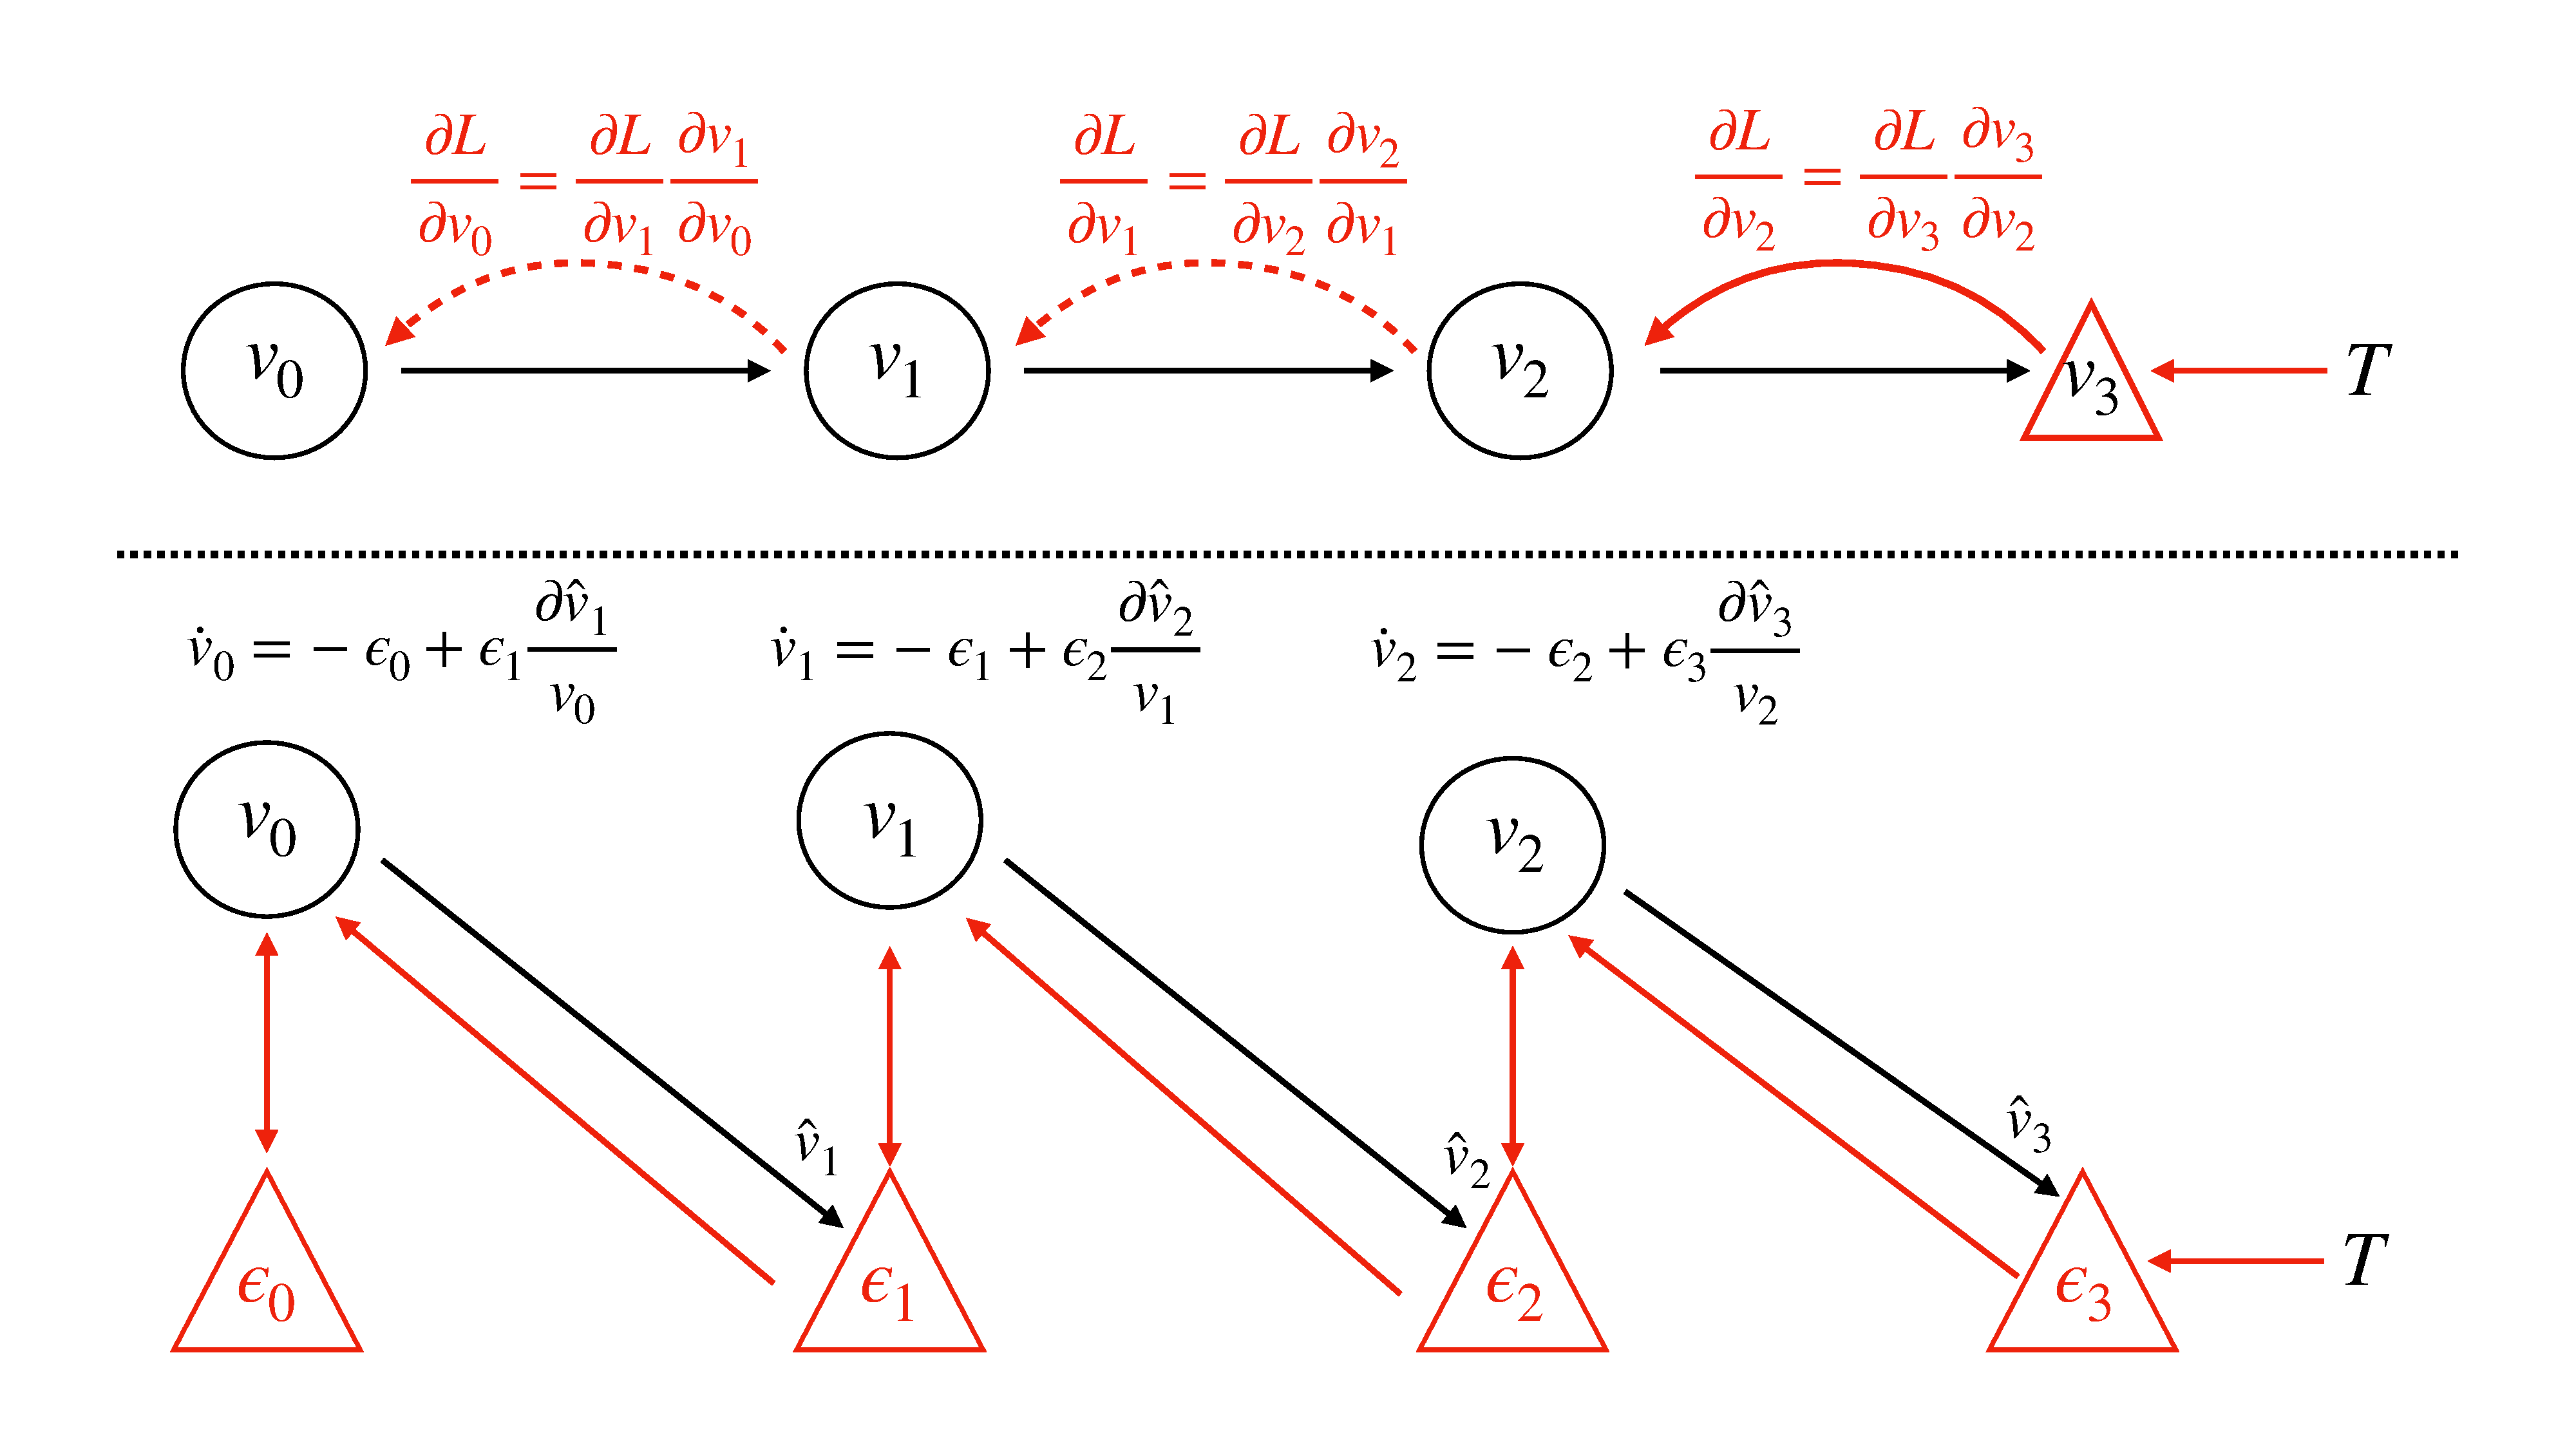
\includegraphics[width=\textwidth]{chapter_6_figures/pc_chain_schematic_new.pdf}
    \caption{Top: Backpropagation on a chain. Backprop proceeds backwawrds sequentially and  explicitly computes the gradient at each step on the chain. Bottom: Predictive coding on a chain.  Predictions, and prediction errors are updated in parallel using only local information.}
\label{main_PCBP_schematic}
\end{figure}

%copied
A computation graph $\mathcal{G} = \{\mathbb{E},\mathbb{V}\}$ is a directed acyclic graph (DAG) which can represent the computational flow of essentially any program or computable function as a composition of elementary functions. Each edge $e_i \in \mathbb{E}$ of the graph corresponds to an intermediate step -- the application of an elementary function -- while each vertex $v_i \in \mathbb{V}$ is an intermediate variable computed by applying the functions of the edges to the values of their originating vertices. $v_i$ denotes the vector of activations within a layer and we denote the set of all vertices as $\{v_i\}$. Effectively, computation flows `forward' from parent nodes to all their children through the edge functions until the leaf nodes give the final output of the program as a whole (see Figure \ref{main_PCBP_schematic} and \ref{PCBP_numerical_results} (top) for an example). Given a target $T$ and a loss function $L = g(T, v_{out})$, the graph's output can be evaluated and, and if every edge function is differentiable, automatic differentiation can be performed on the computation graph.

We can extend predictive coding to arbitrary computation graphs in a supervised setting by defining the inference problem to be solved as that of inferring the vertex value $v_i$ of each node in the graph given fixed start nodes $v_0$ (the data), and end nodes $v_N$ (the targets). We define a generative model which parametrises the value of each vertex given the feedforward prediction of its parents, $p(\{v_i\}) = p(v_0 \dots v_N) = \prod_i^N p(v_i | \mathcal{P}(v_i) )$ \footnote{This includes the prior $p(v_0$), which simply has no parents.}, and a factorised, variational posterior $Q(\{v_i\} | v_0, v_N) = Q(v_1 \dots v_{N-1} | v_0, v_N) = \prod_i^N Q(v_i | \mathcal{P}(v_i), \mathcal{C}(v_i))$, where $\mathcal{P}(v_i)$ denotes the set of parents and $\mathcal{C}(v_i)$ denotes the set of children of a given node $v_i$. From this, we can define a suitable objective functional, the variational free-energy $\mathcal{F}$ (VFE), which acts as an upper bound on the divergence between the true and variational posteriors.
\begin{equation}
\begin{aligned}
    \mathcal{F} &= KL[(Q(v_1 \dots v_{N-1} | v_0, v_N) \Vert p(v_0 \dots v_N)] \geq  KL[(Q(v_1 \dots v_{N-1}) | v_0, v_N) \Vert p(v_1 \dots v_{N-1}| v_0, v_N)] \\
    &\approx \sum_{i=0}^N \epsilon_i^T \epsilon_i 
\end{aligned}
\end{equation}

Under Gaussian assumptions for the generative model $p(\{v_i\}) = \prod_i^N \mathcal{N}(v_i ; \hat{v_i}, \Sigma_i)$, and the variational posterior $Q(\{v_i\}) = \prod_i^N \mathcal{N}(v_i)$, where the `predictions' $\hat{v_i} = f(\mathcal{P}(v_i); \theta_i)$ are defined as the feedforward value of the vertex produced by running the graph forward, and all the precisions, or inverse variances, $\Sigma^{-1}_i$ are fixed at the identity, we can write $\mathcal{F}$ as simply a sum of prediction errors (see chapter 5), with the prediction errors defined as $\epsilon_i = v_i - \hat{v}_i$. Since $\mathcal{F}$ is an upper bound on the divergence between true and approximate posteriors, by minimizing $\mathcal{F}$, we reduce this divergence, thus improving the quality of the variational posterior and approximating exact Bayesian inference. Predictive coding minimizes $\mathcal{F}$ by employing the Cauchy method of steepest descent to set the dynamics of the vertex variables $v_i$ as a gradient descent directly on $\mathcal{F}$

\begin{equation}
\begin{aligned}
\label{PCBP_v_update}
    \frac{dv_i}{dt} = \frac{\partial \mathcal{F}}{\partial v_i} = \epsilon_i - \sum_{j \in \mathcal{C}(v_i)} \epsilon_j \frac{\partial \hat{v}_j}{\partial v_i} 
    \end{aligned}
\end{equation}
The dynamics of the parameters of the edge functions $W$ such that $\hat{v_i} = f(\mathcal{P}(v_i); W)$, can also be derived as a gradient descent on $\mathcal{F}$. In a neural network model, the parameters correspond to the synaptic weights of each layer of the neural network. Importantly these dynamics require only information (the current vertex value, prediction error, and prediction errors of child vertices) locally available at the vertex.
\begin{align*}
\label{PCBP_weight_update}
    \frac{dW_i}{dt} &= \frac{\partial \mathcal{F}}{\partial W_i} = \epsilon_i \frac{\partial \hat{v}_i}{\partial W_i} \numberthis
\end{align*}

To run generalized predictive coding on a given computation graph $\mathcal{G} = \{\mathbb{E},\mathbb{V}\}$, we augment the graph with error units $\epsilon \in \mathcal{E}$ to obtain an augumented computation graph $\tilde{\mathcal{G}} = \{\mathbb{E},\mathbb{V},\mathcal{E} \}$. The predictive coding algorithm then operates in two phases -- a feedforward sweep and a backwards iteration phase. In the feedforward sweep, the augmented computation graph is run forward to obtain the set of predictions $\{ \hat{v_i} \}$, and prediction errors $\{\epsilon_i \} = \{ v_i - \hat{v_i} \}$ for every vertex. To achieve exact equivalence with the backprop gradients computed on the original computation graph, we initialize $v_i = \hat{v}_i$ in the initial feedforward sweep so that the output error computed by the predictive coding network and the original graph are identical -- an assumption we call the \emph{fixed prediction} assumption.

In the backwards iteration phase, the vertex activities $\{ v_i \}$ and prediction errors $\{\epsilon_i \}$ are updated with Equation \ref{PCBP_v_update} for all vertices in parallel until the vertex values converge to a minimum of $\mathcal{F}$. After convergence the parameters are updated according to Equation \ref{PCBP_weight_update}. Note we also assume, following \citet{whittington2017approximation}, that the predictions at each layer are fixed at the values assigned during the feedforward pass throughout the optimisation of the $v$s. We call this the \emph{fixed-prediction assumption}. In effect, by removing the coupling between the vertex activities of the parents and the prediction at the child, this assumption separates the global optimisation problem into a local one for each vertex. We implement these dynamics with a simple forward Euler integration scheme so that the update rule for the vertices became $v_i^{t+1} \leftarrow v_i^t - \eta \frac{d\mathcal{F}}{dv_i^t}$
where $\eta$ is the step-size parameter. Importantly, if the edge function linearly combines the activities and the parameters followed by an elementwise nonlinearity, then both the update rule for the vertices (Equation \ref{PCBP_v_update}) and the parameters (Equation \ref{PCBP_weight_update}) become Hebbian. Specifically, the update rules for the vertices and weights become $\frac{dv_i}{dt} = \epsilon_i - \sum_j \epsilon_j f'(\theta_j \hat{v_j}) \theta_j^T$ and $\frac{d\theta_i}{dt} = \epsilon_i f'(\theta_i \hat{v_i}) \hat{v_i}^T$, respectively.

\begin{algorithm}[H]
\SetAlgoLined
\DontPrintSemicolon
\textbf{Dataset:} $\mathcal{D} = \{\mathbf{X},\mathbf{L}\}$, Augmented Computation Graph $\tilde{\mathcal{G}} = \{\mathbb{E},\mathbb{V},\mathcal{E}\}$, inference learning rate $\eta_v$, weight learning rate $\eta_\theta$
\BlankLine
    \For{$(x,L) \in \mathcal{D}$}{
    $\hat{v_0} \leftarrow x$ \\
    \For{$\hat{v}_i \in \mathbb{V}$}{
    $\hat{v}_i\leftarrow f(\{\mathcal{P}(\hat{v}_i); \theta)$ \\
    }
    $\epsilon_L \leftarrow L - \hat{v}_L$ \\
        \While{not converged}{
        \For{$(v_i, \epsilon_i) \in \tilde{\mathcal{G}}$}{
        $\epsilon_i \leftarrow v_i - \hat{v}_i$ \\
        $v_i^{t+1} \leftarrow v_i^t + \eta_v \frac{d\mathcal{F}}{dv_i^t}$
        }
        }
    \For{$\theta_i \in \mathbb{E}$}{
        $\theta_i^{t+1} \leftarrow \theta_i^t + \eta_\theta \frac{d\mathcal{F}}{d\theta_i^t}$
    }
}

\caption{Generalized Predictive Coding \label{general_alg_pseudocode}}
\end{algorithm}

\section{Methods and Results}

To demonstrate that this predictive coding scheme approximates the backpropagation of error algorithm at convergence is fairly straightforward. The key step is to show that the recursion relationship of the adjoint term for the equilibrium of the prediction errors in predictive coding is identical to that of that in reverse-mode AD, even for arbitrary computation graphs. To make this clear more intuitively, we first demonstrate that, at the equilibrium of the dynamics, the prediction errors $\epsilon^*_i$ converge to the correct backpropagated gradients $\frac{\partial \mathcal{L}}{\partial v_i}$, and consequently the parameter updates (Equation \ref{PCBP_weight_update}) become precisely those of a backprop trained network.

First, under the fixed prediction assumption, we can directly solve for the equilibrium of the dynamics by setting the time derivative to 0,
\begin{align*}
\label{PCBP_error_equilibrium}
    \epsilon_i^* = \sum_{j \in \mathcal{C}(v_i)} \epsilon^*_j \frac{\partial \hat{v}_i}{\partial v_j}
    \numberthis
\end{align*}
If we compare this to the recursive relationship inherent to reverse-mode AD (Equation \ref{reverse_mode_equation}), we can see that the prediction errors satisfy the same recursive relationship. Since this relationship is recursive, all that is needed for the prediction errors throughout the graph to converge to the backpropagated derivatives is for the prediction errors at the final layer to be equal to the output gradient: $\epsilon^*_L = \frac{\partial \mathcal{L}}{\partial \hat{v}_L}$. 
%If this is the case, then due to the recursive structure, the prediction error dynamics converge to the backpropagated gradients at all nodes in the graph.
To see this explicitly, consider a mean-squared-error loss function \footnote{While the mean-squared-error loss function fits most nicely with the Gaussian generative model, other loss functions can be used in practice. If the loss function can be represented as a log probability distribution, then the generative model can be amended to simply set the output distribution to that distribution. If not, then there is no fully consistent generative model (although all nodes except the output remain Gaussian), but the algorithm will still work in practice. See Figure \ref{PCBP_CNN_acc} for results for CNNs trained with a crossentropy loss.}. at the output layer $L = \frac{1}{2}(T - \hat{v}_L)^2$ with T as a vector of targets, and defining $\epsilon_L = T - \hat{v}_L$. We then consider the equilibrium value of the prediction error unit at a penultimate vertex $\epsilon_{L-1}$. By Equation \ref{PCBP_error_equilibrium}, we can see that at equilibrium,
\begin{align*}
    \epsilon^*_{L-1} &= \epsilon^*_L \frac{\partial \hat{v}_L}{\partial v_{L-1}} = (T - \hat{v}_L^*)\frac{\partial \hat{v}_L}{\partial v_{L-1}} \numberthis
\end{align*}
since,  $(T - \hat{v}_L) = \frac{\partial \mathcal{L}}{\partial \hat{v}_L}$, we can then write,
\begin{align*}
     \epsilon^*_{L-1}  &=  \frac{\partial \mathcal{L}}{\partial \hat{v}_L} \frac{\partial \hat{v}_L}{\partial v_{L-1}} =\frac{\partial \mathcal{L}}{\partial v_{L-1}} \numberthis
\end{align*}
Thus the prediction errors of the penultimate nodes converge to the correct backpropagated gradient. Furthermore, recursing through the graph from children to parents allows the correct gradients to be computed\footnote{Some subtlety is needed here since $v_{L-1}$ may have many children which each contribute to the loss. However, these different paths sum together at the node $v_{L-1}$, thus propagating the correct gradient backwards.}. Thus, by induction, we have shown that the fixed points of the prediction errors of the global optimization correspond exactly to the backpropagated gradients. Intuitively, if we imagine the computation-graph as a chain and the error as `tension' in the chain, backprop loads all the tension at the end (the output) and then systematically propagates it backwards. Predictive coding, however, spreads the tension throughout the entire chain until it reaches an equilibrium where the amount of tension at each link is precisely the backpropagated gradient.

By a similar argument, it is apparent that the dynamics of the parameters $\theta_i$ as a gradient descent on $\mathcal{F}$ also exactly match the backpropagated parameter gradients. 
\begin{align*}
    \frac{dW_i}{dt} &= \frac{\partial \mathcal{F}}{\partial W_i} = \epsilon^*_i \frac{\partial \epsilon_i^*}{\partial W_i} \\ 
    &= \frac{\partial \mathcal{L}}{\partial \hat{v}_i} \frac{\partial \hat{v}_i}{\partial  W_i}  
    = \frac{\partial \mathcal{L}}{\partial W_i} \numberthis
\end{align*}
 Which follows from the fact that $\epsilon^*_i = \frac{dL}{d\hat{v}_i}$ and that $\frac{d\epsilon^*_i}{d\theta} = \frac{d \hat{v}_i}{d\theta_i}$.
 
 To demonstrate that empirically that this approach works, we present a numerical test in the simple scalar case, where we use predictive coding to derive the gradients of an arbitrary, highly nonlinear test function $v_{L} = \tan(\sqrt{\theta v_0}) + \sin(v_0^2)$ where $\theta$ is an arbitrary parameter. For our tests, we set $v_0$ to 5 and $\theta$ to 2. The computation graph for this function is presented in Figure \ref{PCBP_numerical_results}. Although simple, this is a good test of predictive coding because the function is highly nonlinear, and its computation graph does not follow a simple layer structure but includes some branching. An arbitrary target of $T = 3$ was set at the output and the gradient of the loss $L= (v_L-T)^2$ with respect to the input $v_0$ was computed by predictive coding. We show (Figure \ref{PCBP_numerical_results}) that the predictive coding optimisation rapidly converges to the exact numerical gradients computed by automatic differentiation, and that moreover this optimization is very robust and can handle even exceptionally high learning rates (up to 0.5) without divergence. 

 \begin{figure}
\begin{subfigure}{\linewidth}
\centering
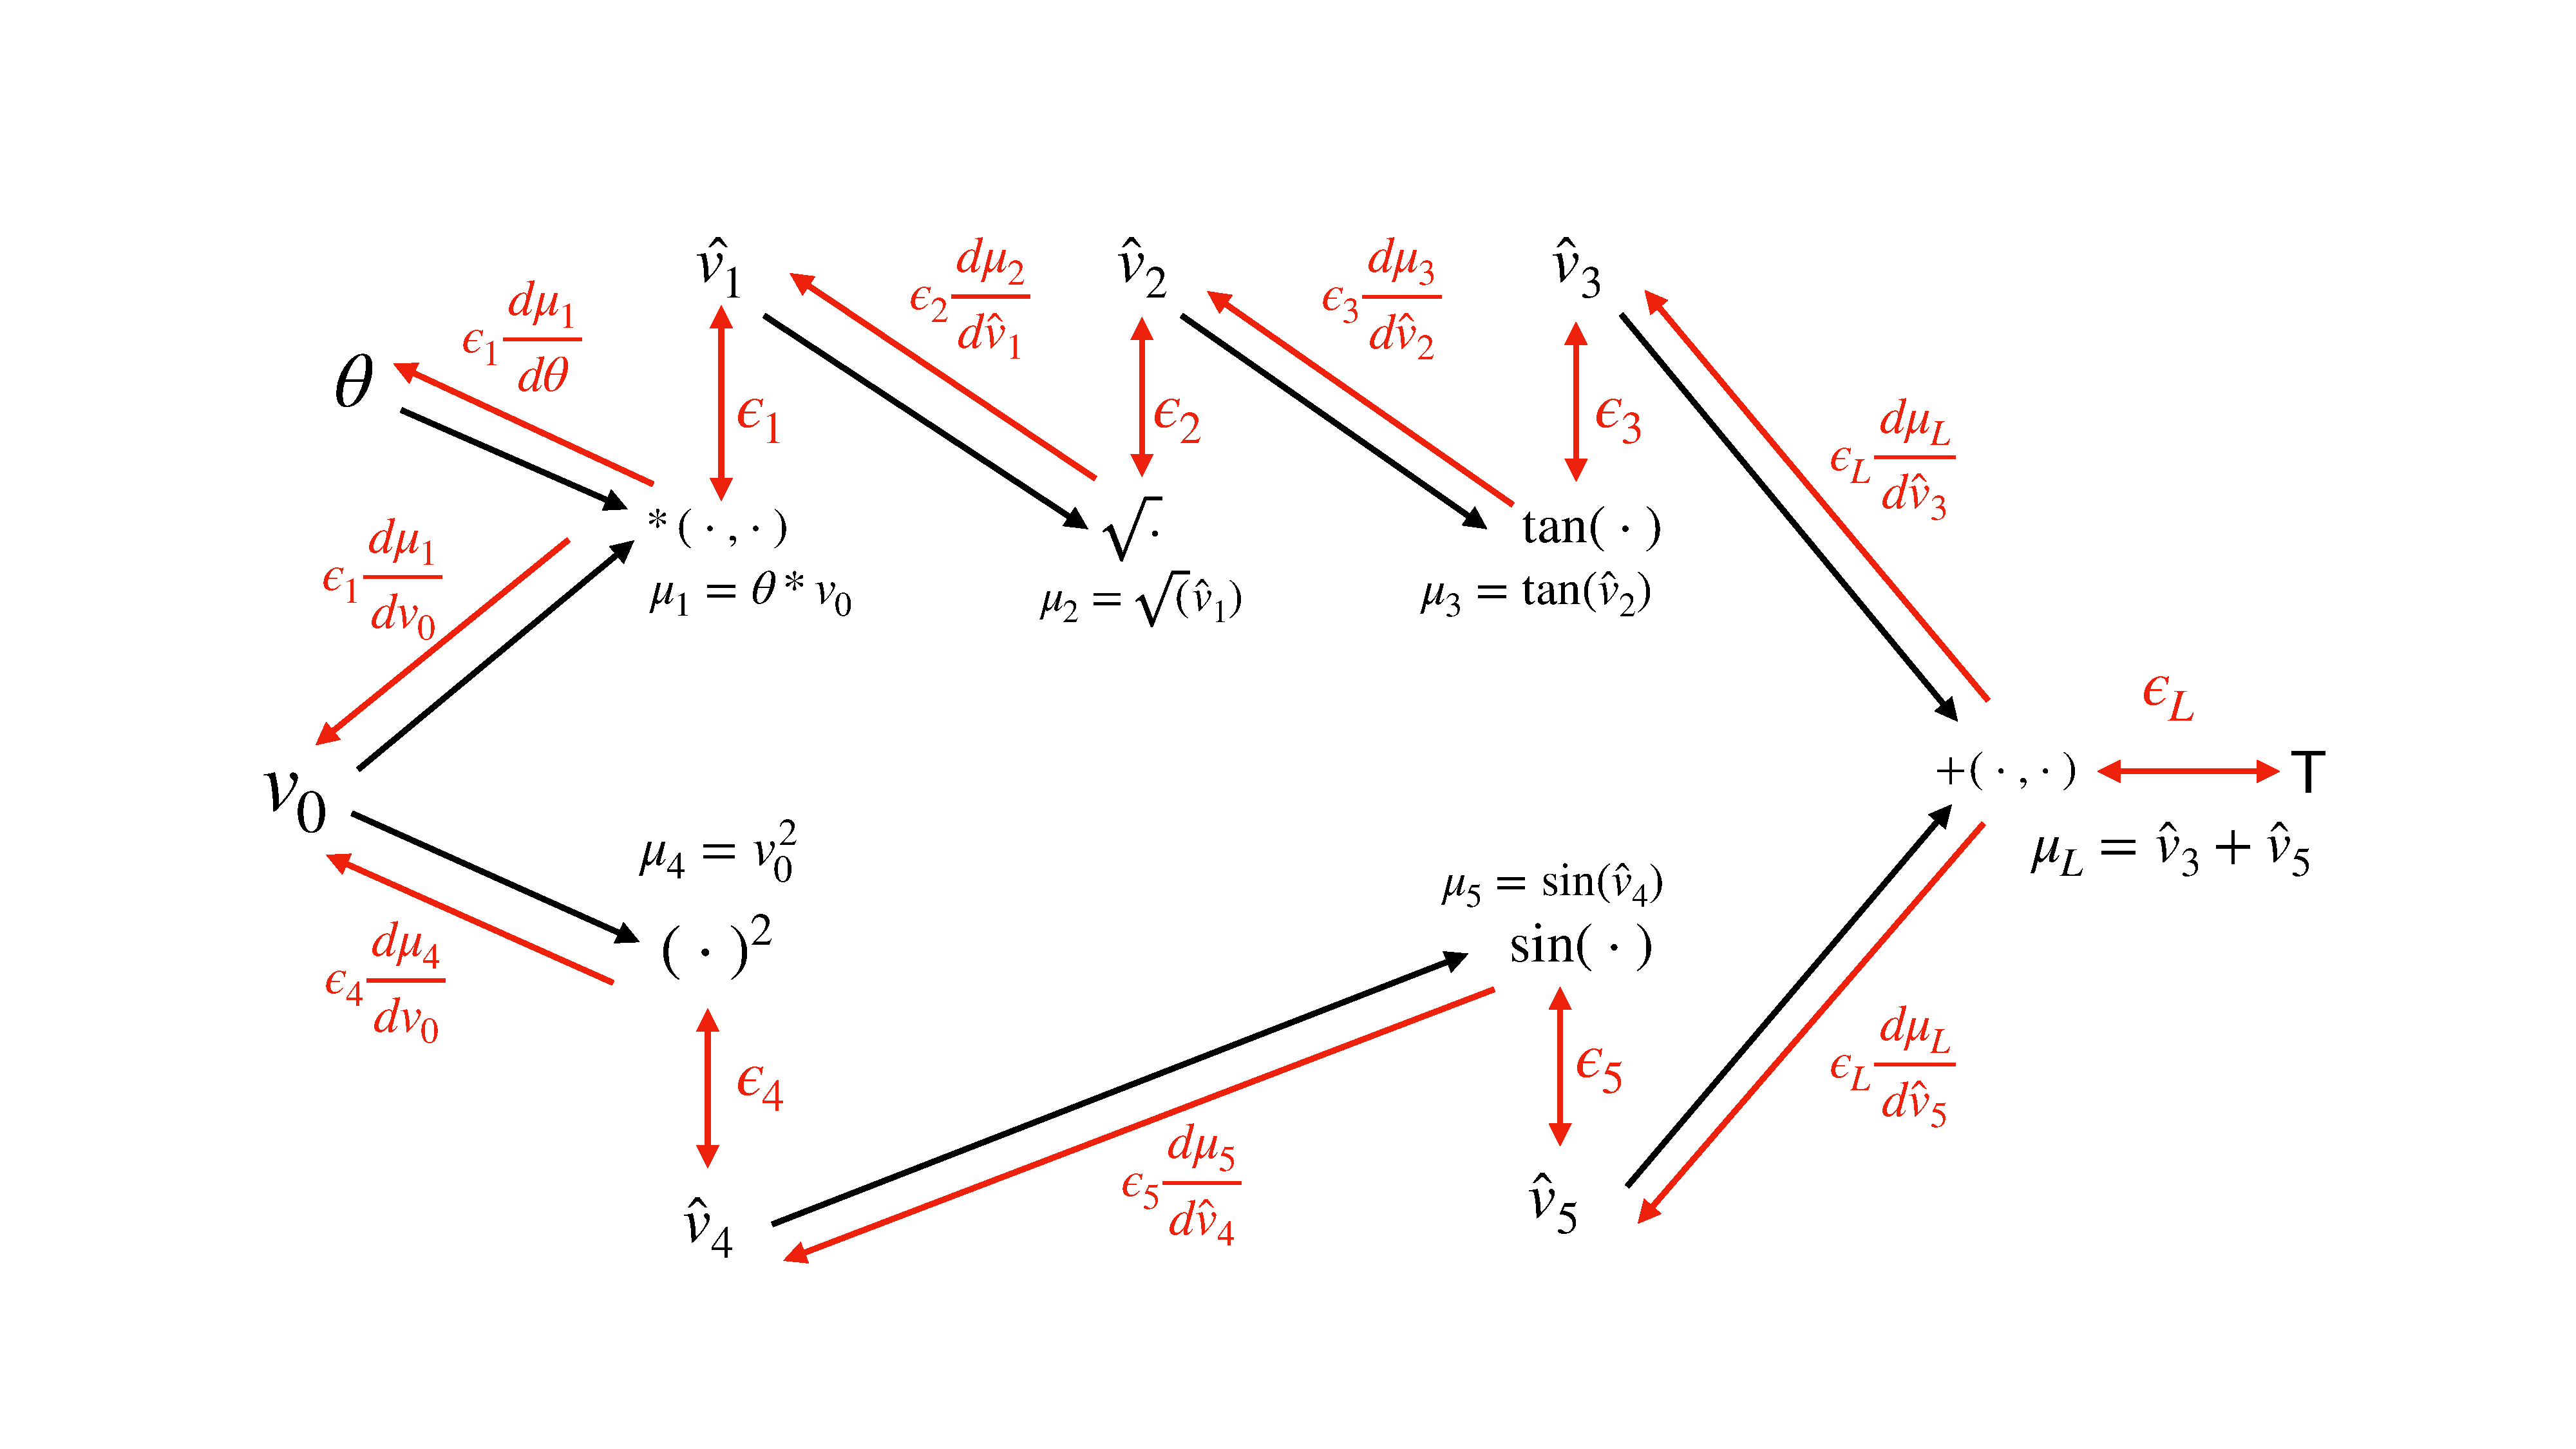
\includegraphics[scale=0.15]{chapter_6_figures/pc_schematic.pdf}
\end{subfigure}
\begin{subfigure}{.5\linewidth}
\centering
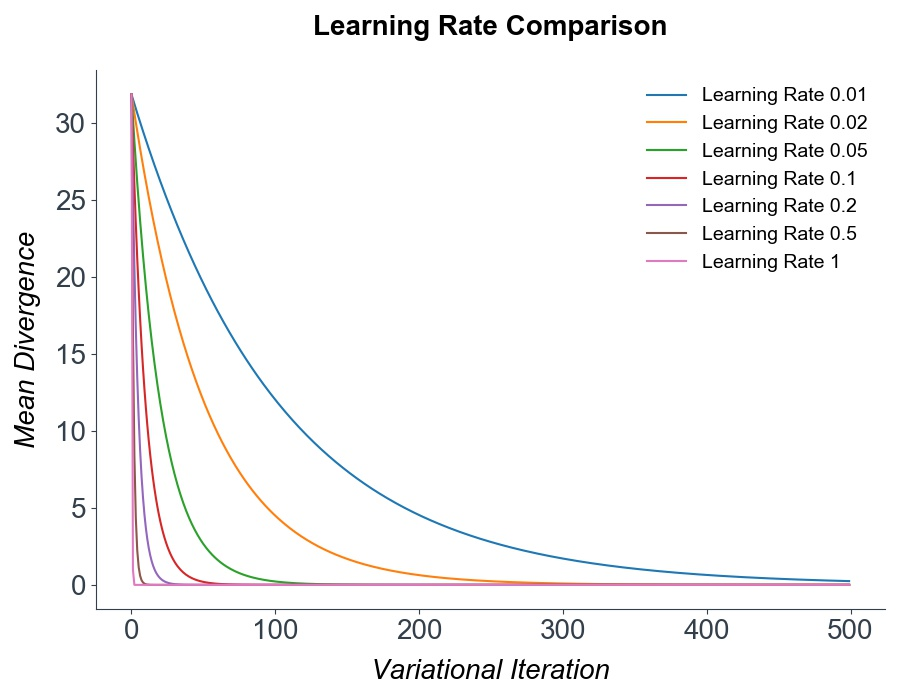
\includegraphics[scale=0.25]{chapter_6_figures/numerics_proper_learning_rate_comparison.jpg}
\end{subfigure}%
\begin{subfigure}{.5\linewidth}
\centering
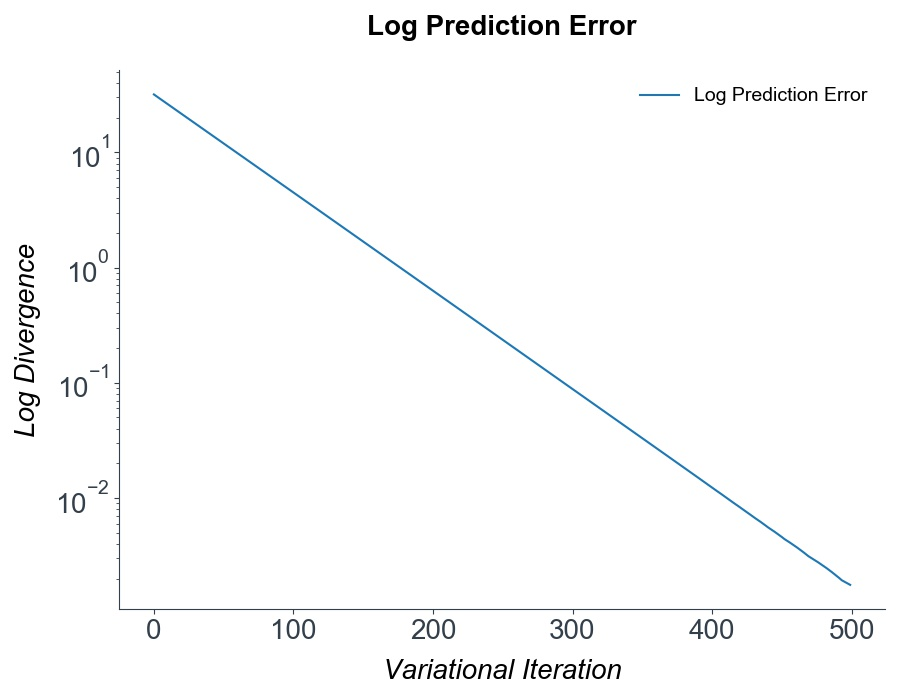
\includegraphics[scale=0.25]{chapter_6_figures/numerics_proper_log_divergence.jpg}
\end{subfigure}\\[1ex]
\caption{Top: The computation graph of the nonlinear test function $v_{L} = \tan(\sqrt{\theta v_0}) + \sin(v_0^2)$. Bottom: graphs of the log mean divergence from the true gradient and the divergence for different learning rates. Convergence to the exact gradients is exponential and robust to high learning rates.}

 \label{PCBP_numerical_results}
\end{figure} \vspace{-0.2cm}

Secondly, we wish to show empirically that this approach can be used to train deep neural network architectures, of the kind used in machine learning, up to high levels of performance equivalent to those trained with backprop. First, we demonstrate a predictive coding CNN model. Convolutional neural networks have been a cornerstone of machine learning since the pioneering demonstrations of their power on ImageNet by \citep{krizhevsky2012imagenet}, and are still widely used as state of the art models for image processing. 

The key concept in a CNN is that of an image convolution, where a small weight matrix is slid (or convolved) across an image to produce an output image. Each patch of the output image only depends on a relatively small patch of the input image. Moreover, the weights of the filter stay the same during the convolution, so each pixel of the output image is generated using the same weights. The weight sharing implicit in the convolution operation enforces translational invariance, since different image patches are all processed with the same weights.

The forward equations of a convolutional layer for a specific output pixel
\begin{align*}
    v_{i,j} = \sum_{k=i-f}^{k=i+f} \sum_{l=j-f}^{l=j+f} \theta_{k,l} x_{i+k,j+l} \numberthis
\end{align*}

Where $v_{i,j}$ is the $(i,j)$th element of the output, $x_{i,j}$ is the element of the input image and $\theta_{k,l}$ is an weight element of a feature map. To setup a predictive coding CNN, we augment each intermediate $x_i$ and $v_i$ with error units $\epsilon_i$ of the same dimension as the output of the convolutional layer.

Predictions $\hat{v}$ are projected forward using the forward equations. Prediction errors also need to be transmitted backwards for the architecture to work. To achieve this we must have that prediction errors are transmitted upwards by a `backwards convolution'. We thus define the backwards prediction errors $\hat{\epsilon}_j$ as follows:
\begin{align*}
    \hat{\epsilon}_{i,j} = \sum_{k=i-f}^{i+f}\sum_{l=j-f}^{j+f} \theta_{j,i} \tilde{\epsilon}_{i,j} \numberthis
\end{align*}

Where $\tilde{\epsilon}$ is an error map zero-padded to ensure the correct convolutional output size. Inference in the predictive coding network then proceeds by updating the intermediate values of each layer as follows:
\begin{align*}
    \frac{dv_l}{dt} = \epsilon_l - \hat{\epsilon}_{l+1} \numberthis
\end{align*}

The CNN weights can be updated using the simple Hebbian rule of the multiplication of the pre and post synaptic potentials. 
\begin{align*}
    \frac{d\theta_l}{dt} = \sum_{i,j} \epsilon_{l_{i,j}} {v_{l-1}}_{i,j}^T  \numberthis
\end{align*}

In our experiments we used a relatively simple CNN architecture consisting of one convolutional layer of kernel size 5, and a filter bank of 6 filters. This was followed by a max-pooling layer with a (2,2) kernel and a further convolutional layer with a (5,5) kernel and filter bank of 16 filters. This was then followed by three fully connected layers of 200, 150, and 10 (or 100 for CIFAR100) output units. Each convolutional and fully connected layer used the relu activation function, except the output layer which was linear. Although this architecture is far smaller than state of the art for convolutional networks, our primary purpose here is to demonstrate the equivalence of predictive coding and backprop. Further work could investigate scaling up predictive coding to more state-of-the-art architectures.

Our datasets consisted of 32x32 RGB images. We normalised the values of all pixels of each image to lie between 0 and 1, but otherwise performed no other image preprocessing. We did not use data augmentation of any kind. We set the weight learning rate for the predictive coding and backprop networks 0.0001. A minibatch size of 64 was used. These parameters were chosen without any detailed hyperparameter search and so are likely suboptimal. The magnitude of the gradient updates was clamped to lie between -50 and 50 in all of our models. This was done to prevent divergences, as occasionally occurred in the LSTM networks, likely due to exploding gradients. 

First, we compare the test and training accuracy, as well as training loss plots for convolutional CNNs trained on CIFAR10. Figure \ref{PCBP_CNN_acc} shows convincingly that the accuracy and indeed the training dynamics of predictive coding and backprop are the same, to all intents and purposes, thus demonstrating that predictive coding approaches can approximate backprop to a very high accuracy, using only local learning rules. To investigate this further, we explicitly plotted the divergence between the gradient estimates produced by predictive coding and the analytically correct gradients produced by backprop.


 \begin{figure*}
        \centering
        \begin{subfigure}[b]{0.475\textwidth}
            \centering
            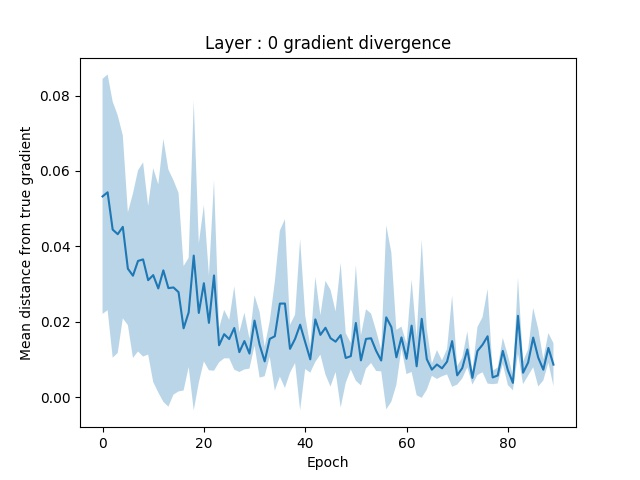
\includegraphics[width=\textwidth]{chapter_6_figures/cnn_weight_diff_0.jpg}
            \caption[Network2]%
            {{\small Conv Layer 1}}    
        \end{subfigure}
        \hfill
        \begin{subfigure}[b]{0.475\textwidth}  
            \centering 
            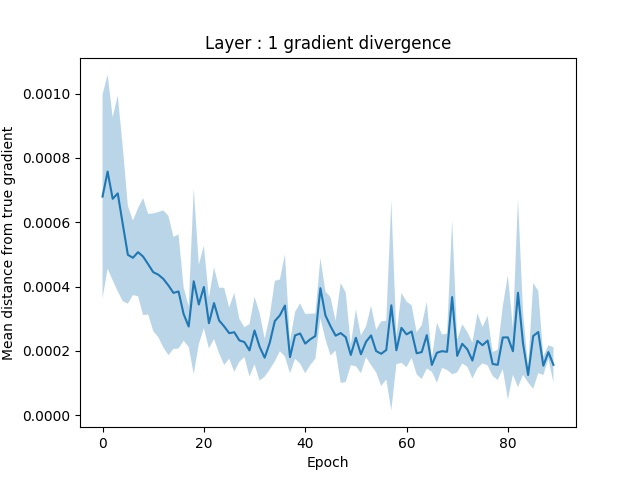
\includegraphics[width=\textwidth]{chapter_6_figures/cnn_weight_diff_1.jpg}
            \caption[]%
            {{\small Conv Layer 2}}    
        \end{subfigure}
        \vskip\baselineskip
        \begin{subfigure}[b]{0.475\textwidth}   
            \centering 
            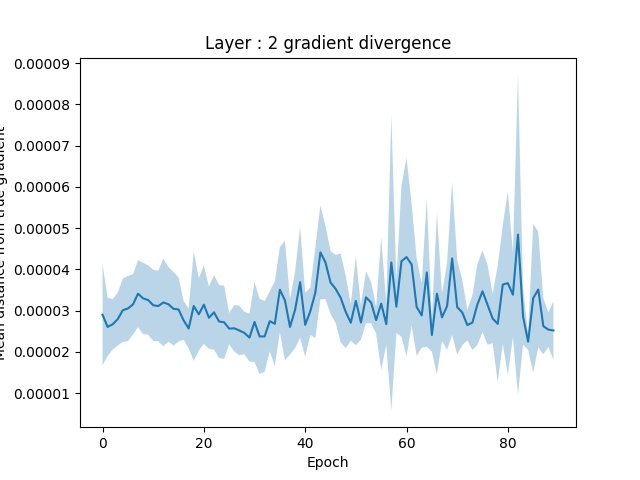
\includegraphics[width=\textwidth]{chapter_6_figures/cnn_weight_diff_2.jpg}
            \caption[]%
            {{\small FC Layer 1}}    
        \end{subfigure}
        \quad
        \begin{subfigure}[b]{0.475\textwidth}   
            \centering 
            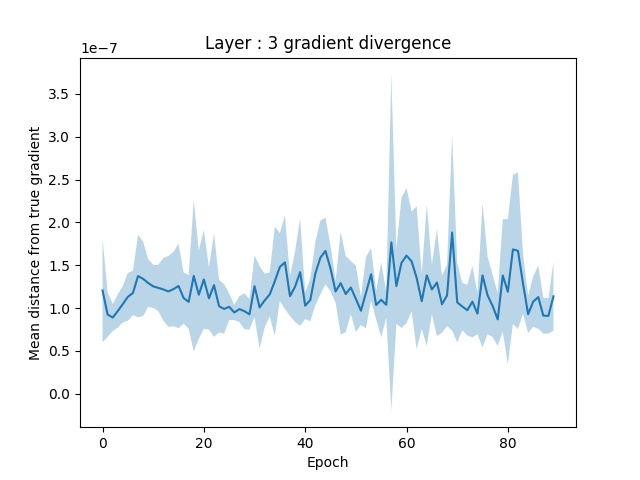
\includegraphics[width=\textwidth]{chapter_6_figures/cnn_weight_diff_3.jpg}
            \caption[]
            {{\small FC Layer 2}}    
        \end{subfigure}
        \caption{\small Mean divergence between the true numerical and predictive coding backprops over the course of training. In general, the divergence appeared to follow a largely random walk pattern, and was generally neglible. Importantly, the divergence did not grow over time throughout training, implying that errors from slightly incorrect gradients did not appear to compound.} 
       
\label{training_divergence}
    \end{figure*}
    
Importantly, we found that the divergence between the true and predictive coding gradients was extremely small, and remained approximately constant throughout training suggesting that predictive coding networks do not suffer from accumulating errors in their gradient approximation process. Importantly, to achieve this level of convergence required 100 backwards iterations using an inference learning rate of 0.1. This means that the predictive coding has an approximately 100x computational overhead compared to backprop -- largely rendering it uncompetitive for direct competition in serial computers. Nevertheless, this choice of 100 iterations is on the high end of what is necessary, since we are primarily concerned with showing the asymptotic equivalence, and in reality the number of iterations required may be substantially lower. Additionally, predictive coding is a fully parallel algorithm unlike backprop, which must be implemented sequentially and is a better fit for the highly parallel neural circuitry.

It is also important to note that while predictive coding `naturally' uses the mean-squared error loss -- so that the output error is a standard prediction error, other loss functions as possible, such as the widely used cross-entropy loss. Predictive coding can be straightforwardly extended to cover other loss functions by simply replacing the final prediction error $\epsilon_L$ with the gradient of the loss function with respect to the outputs.  Here we demonstrate that predictive coding with a multi-class cross entropy loss also performs equivalently to the network trained with backprop on the CIFAR and SVHN datasets.

 \begin{figure*}
        \centering
        \begin{subfigure}[b]{0.475\textwidth}
            \centering
            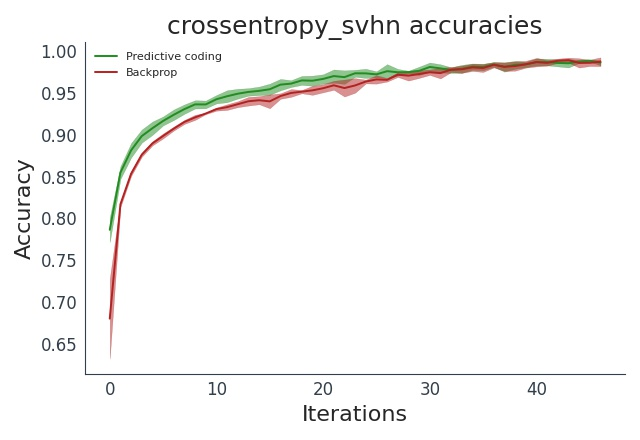
\includegraphics[width=\textwidth]{chapter_6_figures/crossentropy_svhn_accuracies_prelim_2.jpg}

            {{\small SVHN training accuracy }}    
        \end{subfigure}
        \hfill
        \begin{subfigure}[b]{0.475\textwidth}  
            \centering 
            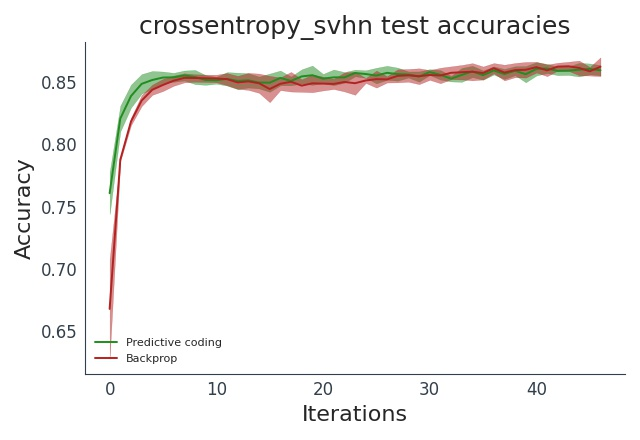
\includegraphics[width=\textwidth]{chapter_6_figures/crossentropy_svhn_test accuracies_prelim_2.jpg}
            \caption[]%
            {{\small SVHN test accuracy}}    
        \end{subfigure}
        \vskip\baselineskip
        \begin{subfigure}[b]{0.475\textwidth}   
            \centering 
            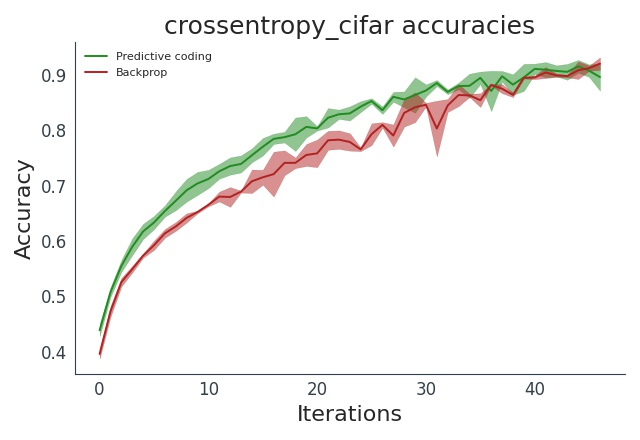
\includegraphics[width=\textwidth]{chapter_6_figures/crossentropy_cifar_accuracies_prelim_2.jpg}
            \caption[]%
            {{\small CIFAR training accuracy}}    
        \end{subfigure}
        \quad
        \begin{subfigure}[b]{0.475\textwidth}   
            \centering 
            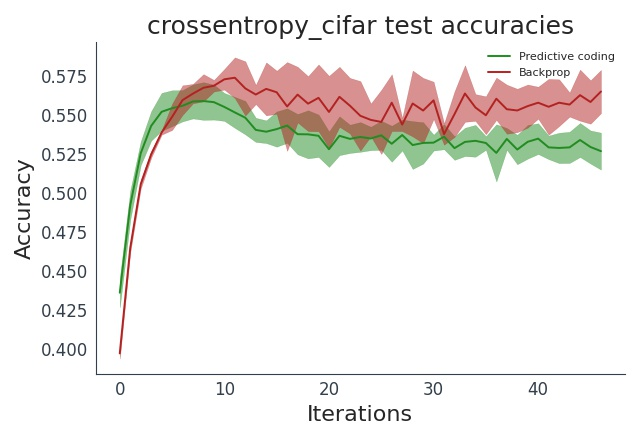
\includegraphics[width=\textwidth]{chapter_6_figures/crossentropy_cifar_test accuracies_prelim_2.jpg}
            \caption[]
            {{\small CIFAR test accuracy}}    
        \end{subfigure}
        \caption{\small Training and test accuracies of the CNN network on the SVHN and CIFAR datasets using the cross-entropy loss. As can be seen performance remains very close to backprop, thus demonstrating that our predictive coding algorithm can be used with different loss functions, not just mean-squared-error.} 
       
        \label{PCBP_CNN_acc}
    \end{figure*}

\subsection{RNN and LSTM}
\subsubsection{RNN}
We additionally tested a predictive coding RNN and LSTM. To train these recurrent networks with predictive coding, we simply used the approach of using predictive coding to approximate backpropagation through time (BPTT) and applied predictive coding to the unrolled computation graph. With long sequence lengths, this lead to extremely deep graphs for predictive coding to train. Crucially, we demonstrate that predictive coding's ability to train such graphs is not impaired by their depth, meaning that predictive coding as a training algorithm has an exceptional scalability for extremely deep models of the kind increasingly used in contemporary machine learning \citep{radford2019language,he2016deep}


The computation graph on RNNs is relatively straightforward. We consider only a single layer RNN here although the architecture can be straightforwardly extended to hierarchically stacked RNNs. An RNN is similar to a feedforward network except that it possesses an additional hidden state $h$ which is maintained and updated over time as a function of both the current input $x$ and the previous hidden state. The output of the network $y$ is a function of $h$. By considering the RNN at a single timestep we obtain the following equations.
\begin{align*}
    \numberthis
    h_t &= f(\theta_h h_{t-1} + \theta_x x_t) \\
    y_t &= g(\theta_y h_t) \numberthis
\end{align*}
Where f and g are elementwise nonlinear activation functions. And $\theta_h, \theta_x, \theta_y$ are weight matrices for each specific input. To predict a sequence the RNN simply rolls forward the above equations to generate new predictions and hidden states at each timestep.

It is important to note that this is an additional aspect of biological implausibility that we do not address in here. BPTT requires updates to proceed backwards through time from the end of the sequence to the beginning. Ignoring any biological implausibility with the rules themselves, this updating sequence is clearly not biologically plausible as naively it requires maintaining the entire sequence of predictions and prediction errors perfectly in memory until the end of the sequence, and waiting until the sequence ends before making any updates. There is a small literature on trying to produce biologically plausible, or forward-looking approximations to BPTT which does not require updates to be propagated back through time \citep{williams1989learning,lillicrap2019backpropagation,steil2004backpropagation,ollivier2015training,tallec2017unbiased}. While this is a fascinating area, we do not address it here. We are solely concerned with the fact that predictive coding approximates backpropagation on feedforward computation graphs for which the unrolled RNN graph is a sufficient substrate.

To learn a predictive coding RNN, we first augment each of the variables $h_t$ and $y_t$ of the original graph with additional error units $\epsilon_{h_t}$ and $\epsilon_{y_t}$. Predictions $\hat{y}_t, \hat{h}_t$ are generated according to the feedforward rules (16). A sequence of true labels $\{T_1...T_T\}$ is then presented to the network, and then inference proceeds by recursively applying the following rules backwards through time until convergence.
\begin{align*}
    \epsilon_{y_t} &= L - \hat{y}_{t} \\
    \epsilon_{h_t} &= h_t - \hat{h}_{t} \\
    \frac{dh_t}{dt} &= \epsilon_{h_t} - \epsilon_{y_t} \theta_y^T - \epsilon_{h_{t+1}} \theta_h^T \numberthis
\end{align*}

Upon convergence the weights are updated according to the following rules.
\begin{align*}
    \frac{d\theta_y}{dt} &= \sum_{t=0}^T \epsilon_{y_t} \frac{\partial g(\theta_y h_t)}{\partial \theta_y} h_t^T \\
    \frac{d\theta_x}{dt} &= \sum_{t=0}^T \epsilon_{h_t} \frac{\partial f(\theta_h h_{t-1}+\theta_x x_t)}{\partial \theta_x} x_t^T \\
    \frac{d\theta_h}{dt} &= \sum_{t=0}^T \epsilon_{h_t} \frac{\partial f(\theta_h h_{t-1}+\theta_x x_t)}{\partial \theta_h} h_{t+1}^T \numberthis
\end{align*}

Since the RNN feedforward updates are parameter-linear, these rules are Hebbian, only requiring the multiplication of pre and post-synaptic potentials. This means that the predictive coding updates proposed here are biologically plausible and could in theory be implemented in the brain. The only biological implausibility remains the BPTT learning scheme.

Our RNN was trained on a simple character-level name-origin dataset which can be found here: \textit{https://download.pytorch.org/tutorial/data.zip}. The RNN was presented with sequences of characters representing names and had to predict the national origin of the name -- French, Spanish, Russian, etc. The characters were presented to the network as one-hot-encoded vectors without any embedding. The output categories were also presented as a one-hot vector. The RNN has a hidden size of 256 units. A \textit{tanh} nonlinearity was used between hidden states and the output layer was linear. The network was trained on randomly selected name-category pairs from the dataset. 

We first present the training and test accuracy for the backprop RNNs, averaged over five seeds. In general, performance between the backprop-trained and predictive coding networks was indistinguishable on this task.

\begin{figure}[ht]
\vspace{-0.3cm}
\hspace{-0.6cm}
\begin{subfigure}{.5\textwidth}
  \centering
  % include first image
  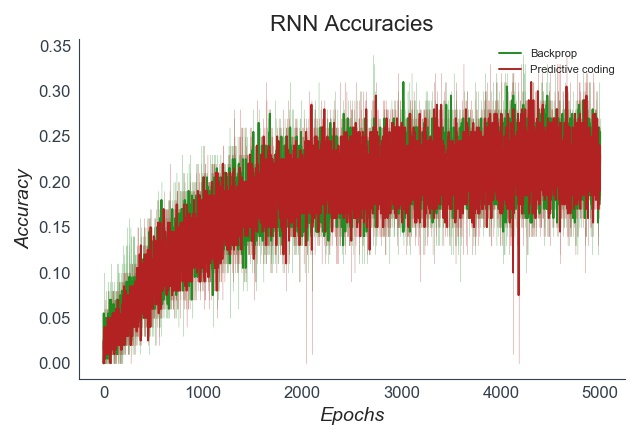
\includegraphics[width=1\linewidth]{chapter_6_figures/RNN_Accuracies_super_prelim_6.jpg}  
  %\caption{SVHN Training Accuracy}
\end{subfigure}
\begin{subfigure}{.5\textwidth}
  \centering
  % include second image
  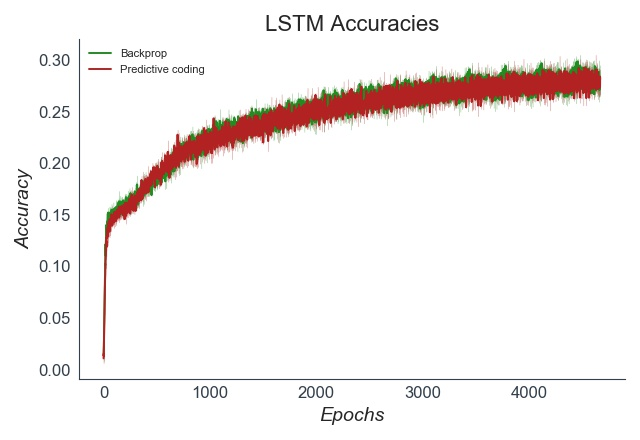
\includegraphics[width=1\linewidth]{chapter_6_figures/LSTM_Accuracies_super_prelim_6.jpg}  
  %\caption{CIFAR10 Training Accuracy}
\end{subfigure}
\caption{Test accuracy plots for the Predictive Coding and Backprop RNN and LSTM on their respective tasks, averaged over 5 seeds. Performance is again indistinguishable from backprop.}

\label{pc_rnn_lstm_results_figure}
\vspace{-0.3cm}
\end{figure}

Additionally, The training loss for the predictive coding and backprop RNNs, averaged over 5 seeds is presented below (Figure \ref{rnn_losses}).

\begin{figure}[ht]
  \centering
  % include first image
  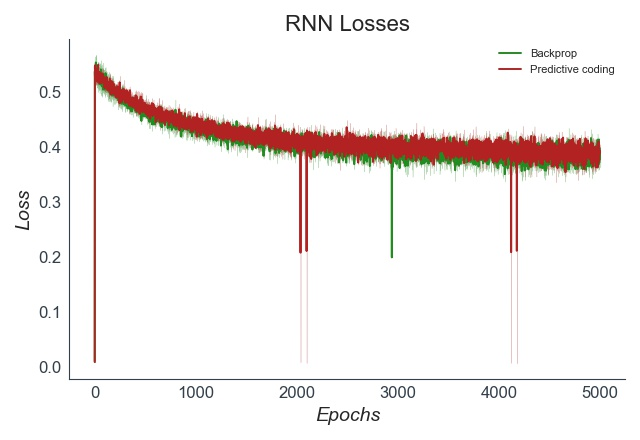
\includegraphics[width=.7\linewidth]{chapter_6_figures/RNN_Losses_super_prelim_6.jpg}  
\caption{Training losses for the predictive coding and backprop RNN. As expected, they are effectively identical.}

\label{rnn_losses}
\end{figure}
\subsubsection{LSTM}
\begin{figure}[ht]
  \centering
  % include first image
  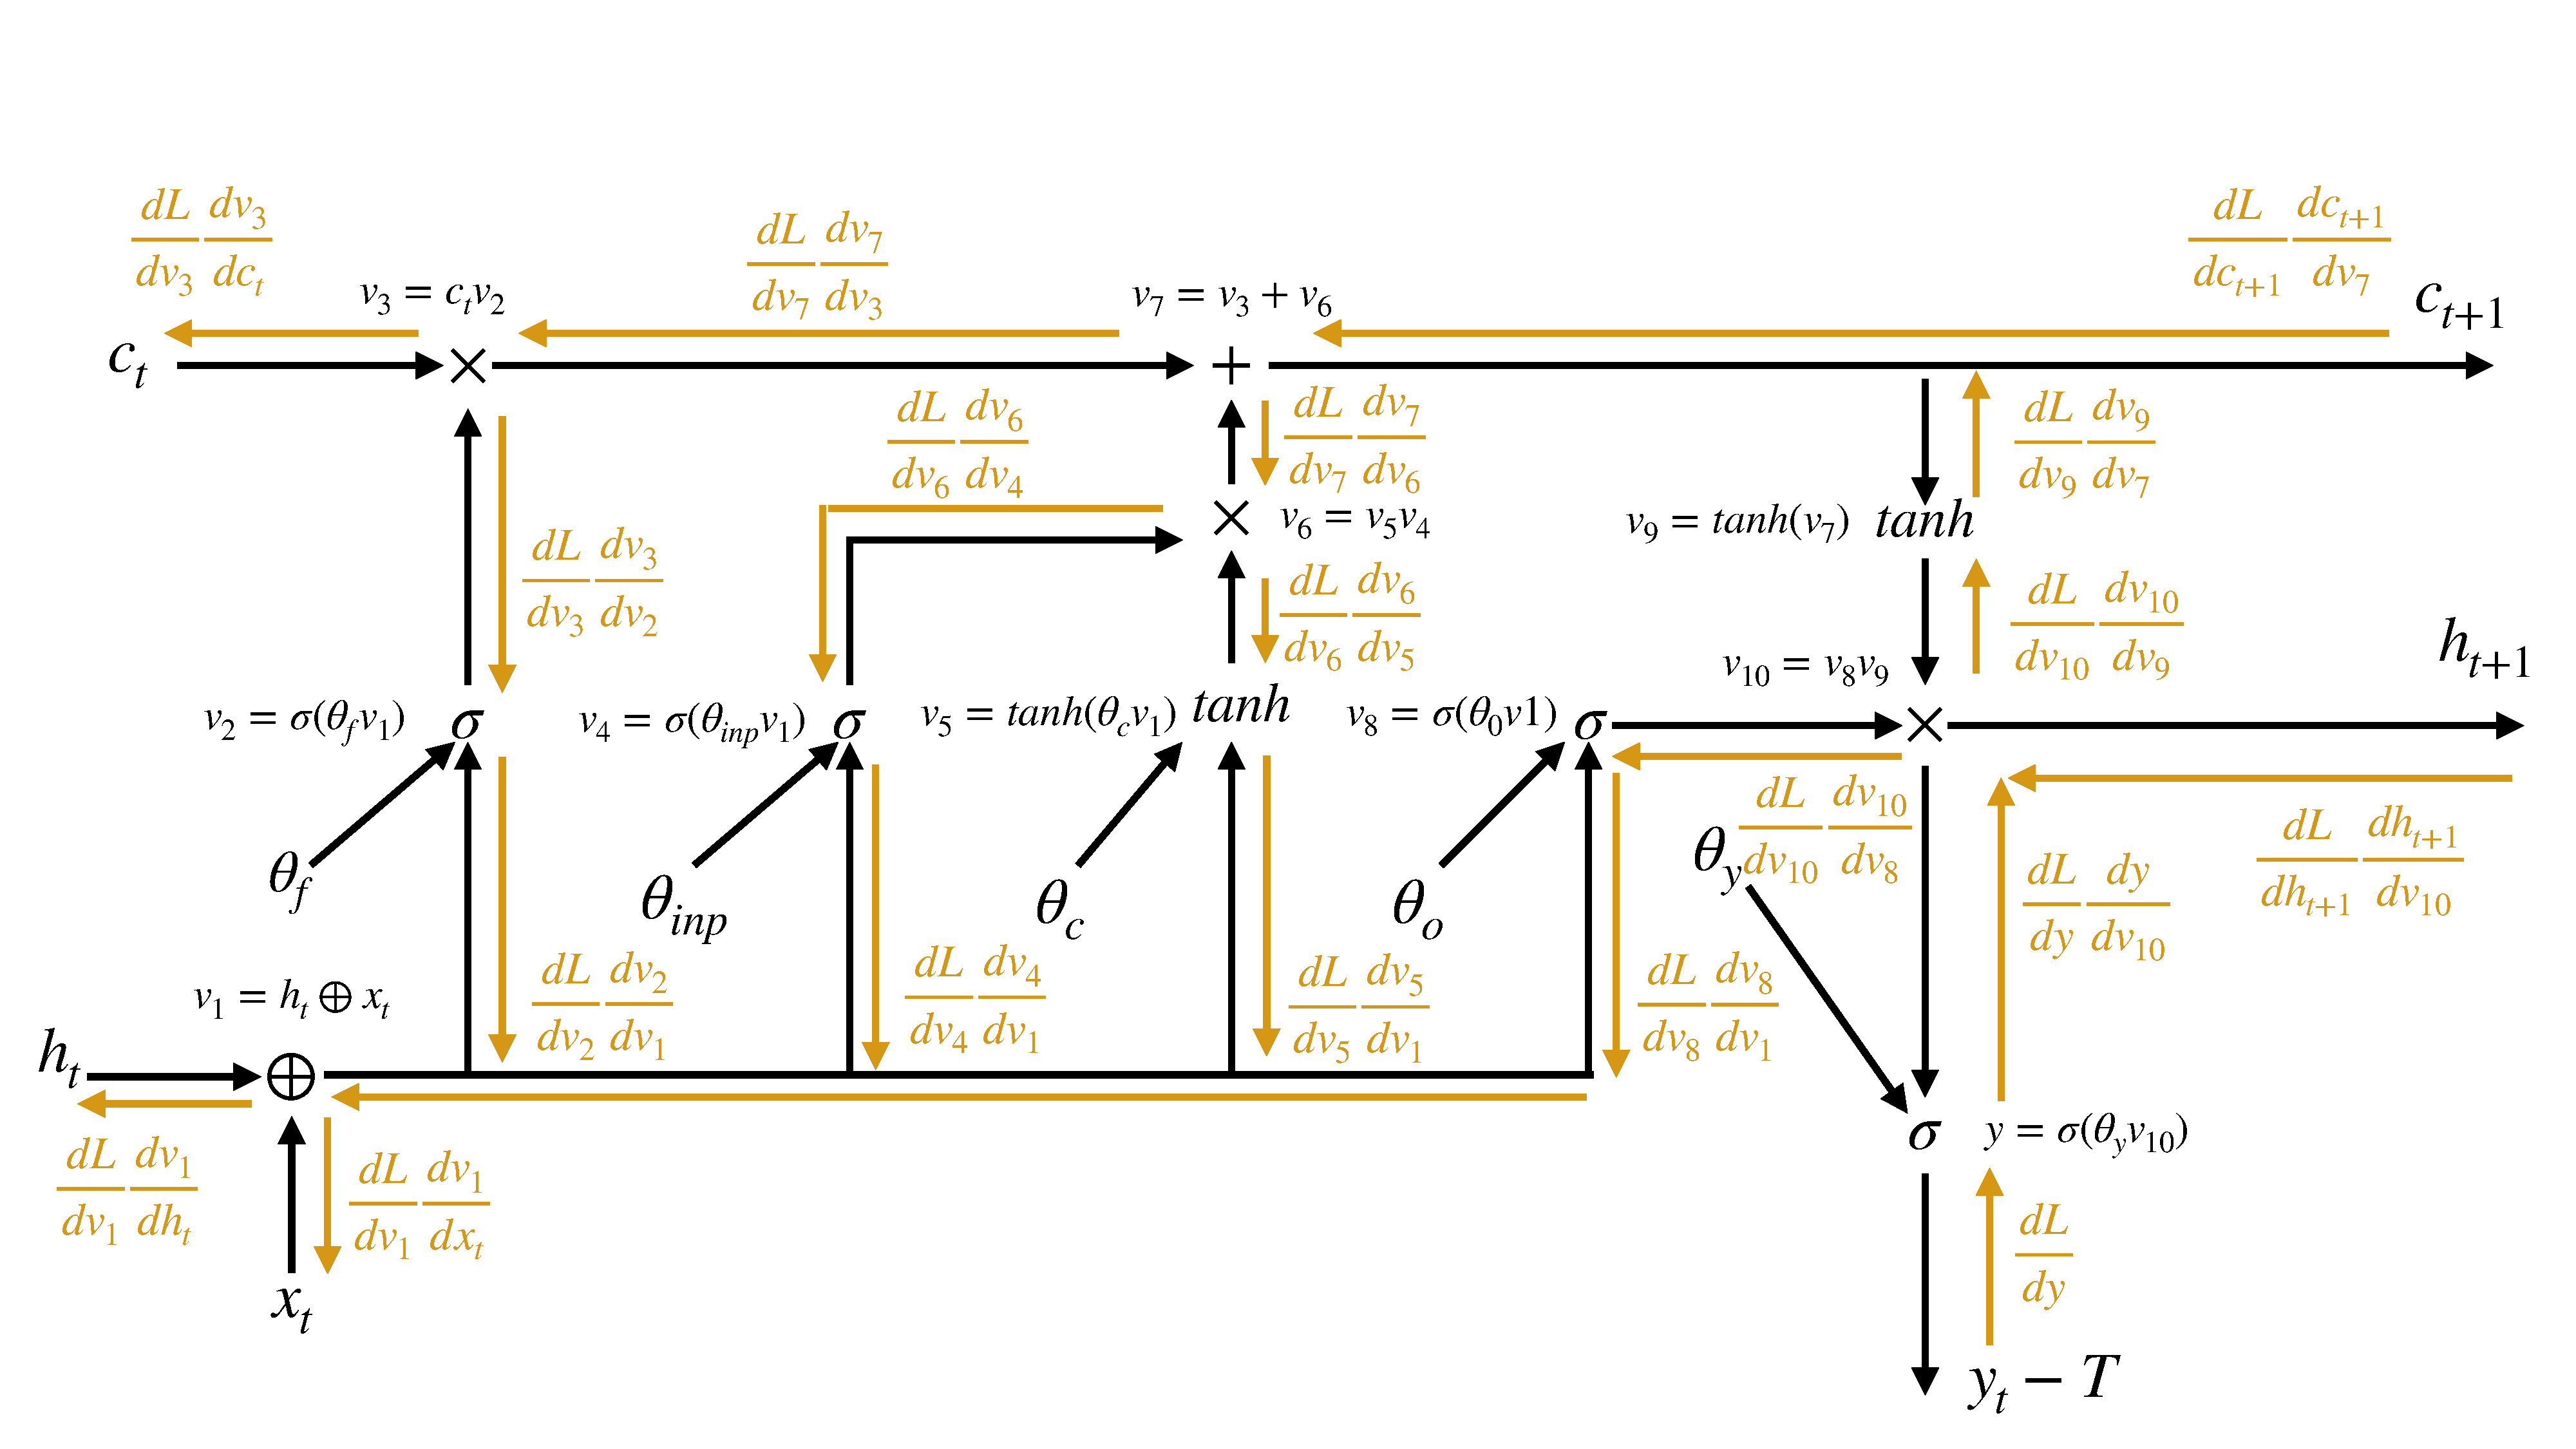
\includegraphics[width=1\linewidth]{chapter_6_figures/backprop_LSTM.pdf}  
\caption{Computation graph and backprop learning rules for a single LSTM cell.}

\label{PC_LSTM}
\end{figure}
Unlike the other two models, the LSTM possesses a complex and branching internal computation graph, and is thus a good opportunity to make explicit the predictive coding `recipe' for approximating backprop on arbitrary computation graphs. The computation graph for a single LSTM cell is shown (with backprop updates) in Figure \ref{pc_lstm}. Prediction for the LSTM occurs by simply rolling forward a copy of the LSTM cell for each timestep. The LSTM cell receives its hidden state $h_t$ and cell state $c_t$ from the previous timestep. During training we compute derivatives on the unrolled computation graph and receive backwards derivatives (or prediction errors) from the LSTM cell at time $t+1$.

The equations that specify the computation graph of the LSTM cell are as follows.
\begin{align*}
    v_1 &= h_t \oplus x_t \\
    v_2 &= \sigma(\theta_i v_1) \\ 
    v_3 &= c_t v_2 \\ 
    v_4 &= \sigma (\theta_{inp} v_1) \\ 
    v_5 &= \tanh(\theta_c v_1) \\ 
    v_6 &= v_4 v_5 \\ 
    v_7 &= v_3 + v_6 \\ 
    v_8 &= \sigma (\theta_o v_1)  \\ 
    v_9 &= \tanh(v_7)\\
    v_{10} &= v_8 v_9 \\
    y &= \sigma(\theta_y v_{10})
\end{align*}

The recipe to convert this computation graph into a predictive coding algorithm is straightforward. We first rewire the connectivity so that the predictions are set to the forward functions of their parents. We then compute the errors between the vertices and the predictions. 
\begin{align*}
    \hat{v}_1 &= h_t \oplus x_t \\
    \hat{v}_2 &= \sigma(\theta_i v_1) \\ 
    \hat{v}_3 &= c_t v_2 \\ 
    \hat{v}_4 &= \sigma (\theta_{inp} v_1) \\ 
    \hat{v}_5 &= \tanh(\theta_c v_1) \\ 
    \hat{v}_6 &= v_4 v_5 \\ 
    \hat{v}_7 &= v_3 + v_6 \\ 
    \hat{v} &= \sigma (\theta_o v_1)  \\ 
    \hat{v}_9 &= \tanh(v_7)\\
    \hat{v}_{10} &= v_8 v_9 \\
    \hat{v}_y &= \sigma(\theta_y v_{10}) \\
    \epsilon_1 &= v_1 - \hat{v}_1 \\
    \epsilon_2 &= v_2 - \hat{v}_2 \\
    \epsilon_3 &= v_3 - \hat{v}_3 \\
    \epsilon_4 &= v_4 - \hat{v}_4 \\
    \epsilon_5 &= v_5 - \hat{v}_5 \\
    \epsilon_6 &= v_6 - \hat{v}_6 \\
    \epsilon_7 &= v_7 - \hat{v}_7 \\
    \epsilon_8 &= v_8 - \hat{v}_8 \\
    \epsilon_9 &= v_9 - \hat{v}_9 \\
    \epsilon_{10} &= v_{10} - \hat{v}_{10}
\end{align*}

During inference, the inputs $h_t$,$x_t$ and the output $y_t$ are fixed. The vertices and then the prediction errors are updated. This recipe is straightforward and can easily be extended to other more complex machine learning architectures. The full augmented computation graph, including the vertex update rules, is presented in Figure \ref{PC_LSTM}.


\begin{figure}%[ht]
  \centering
  % include first image
  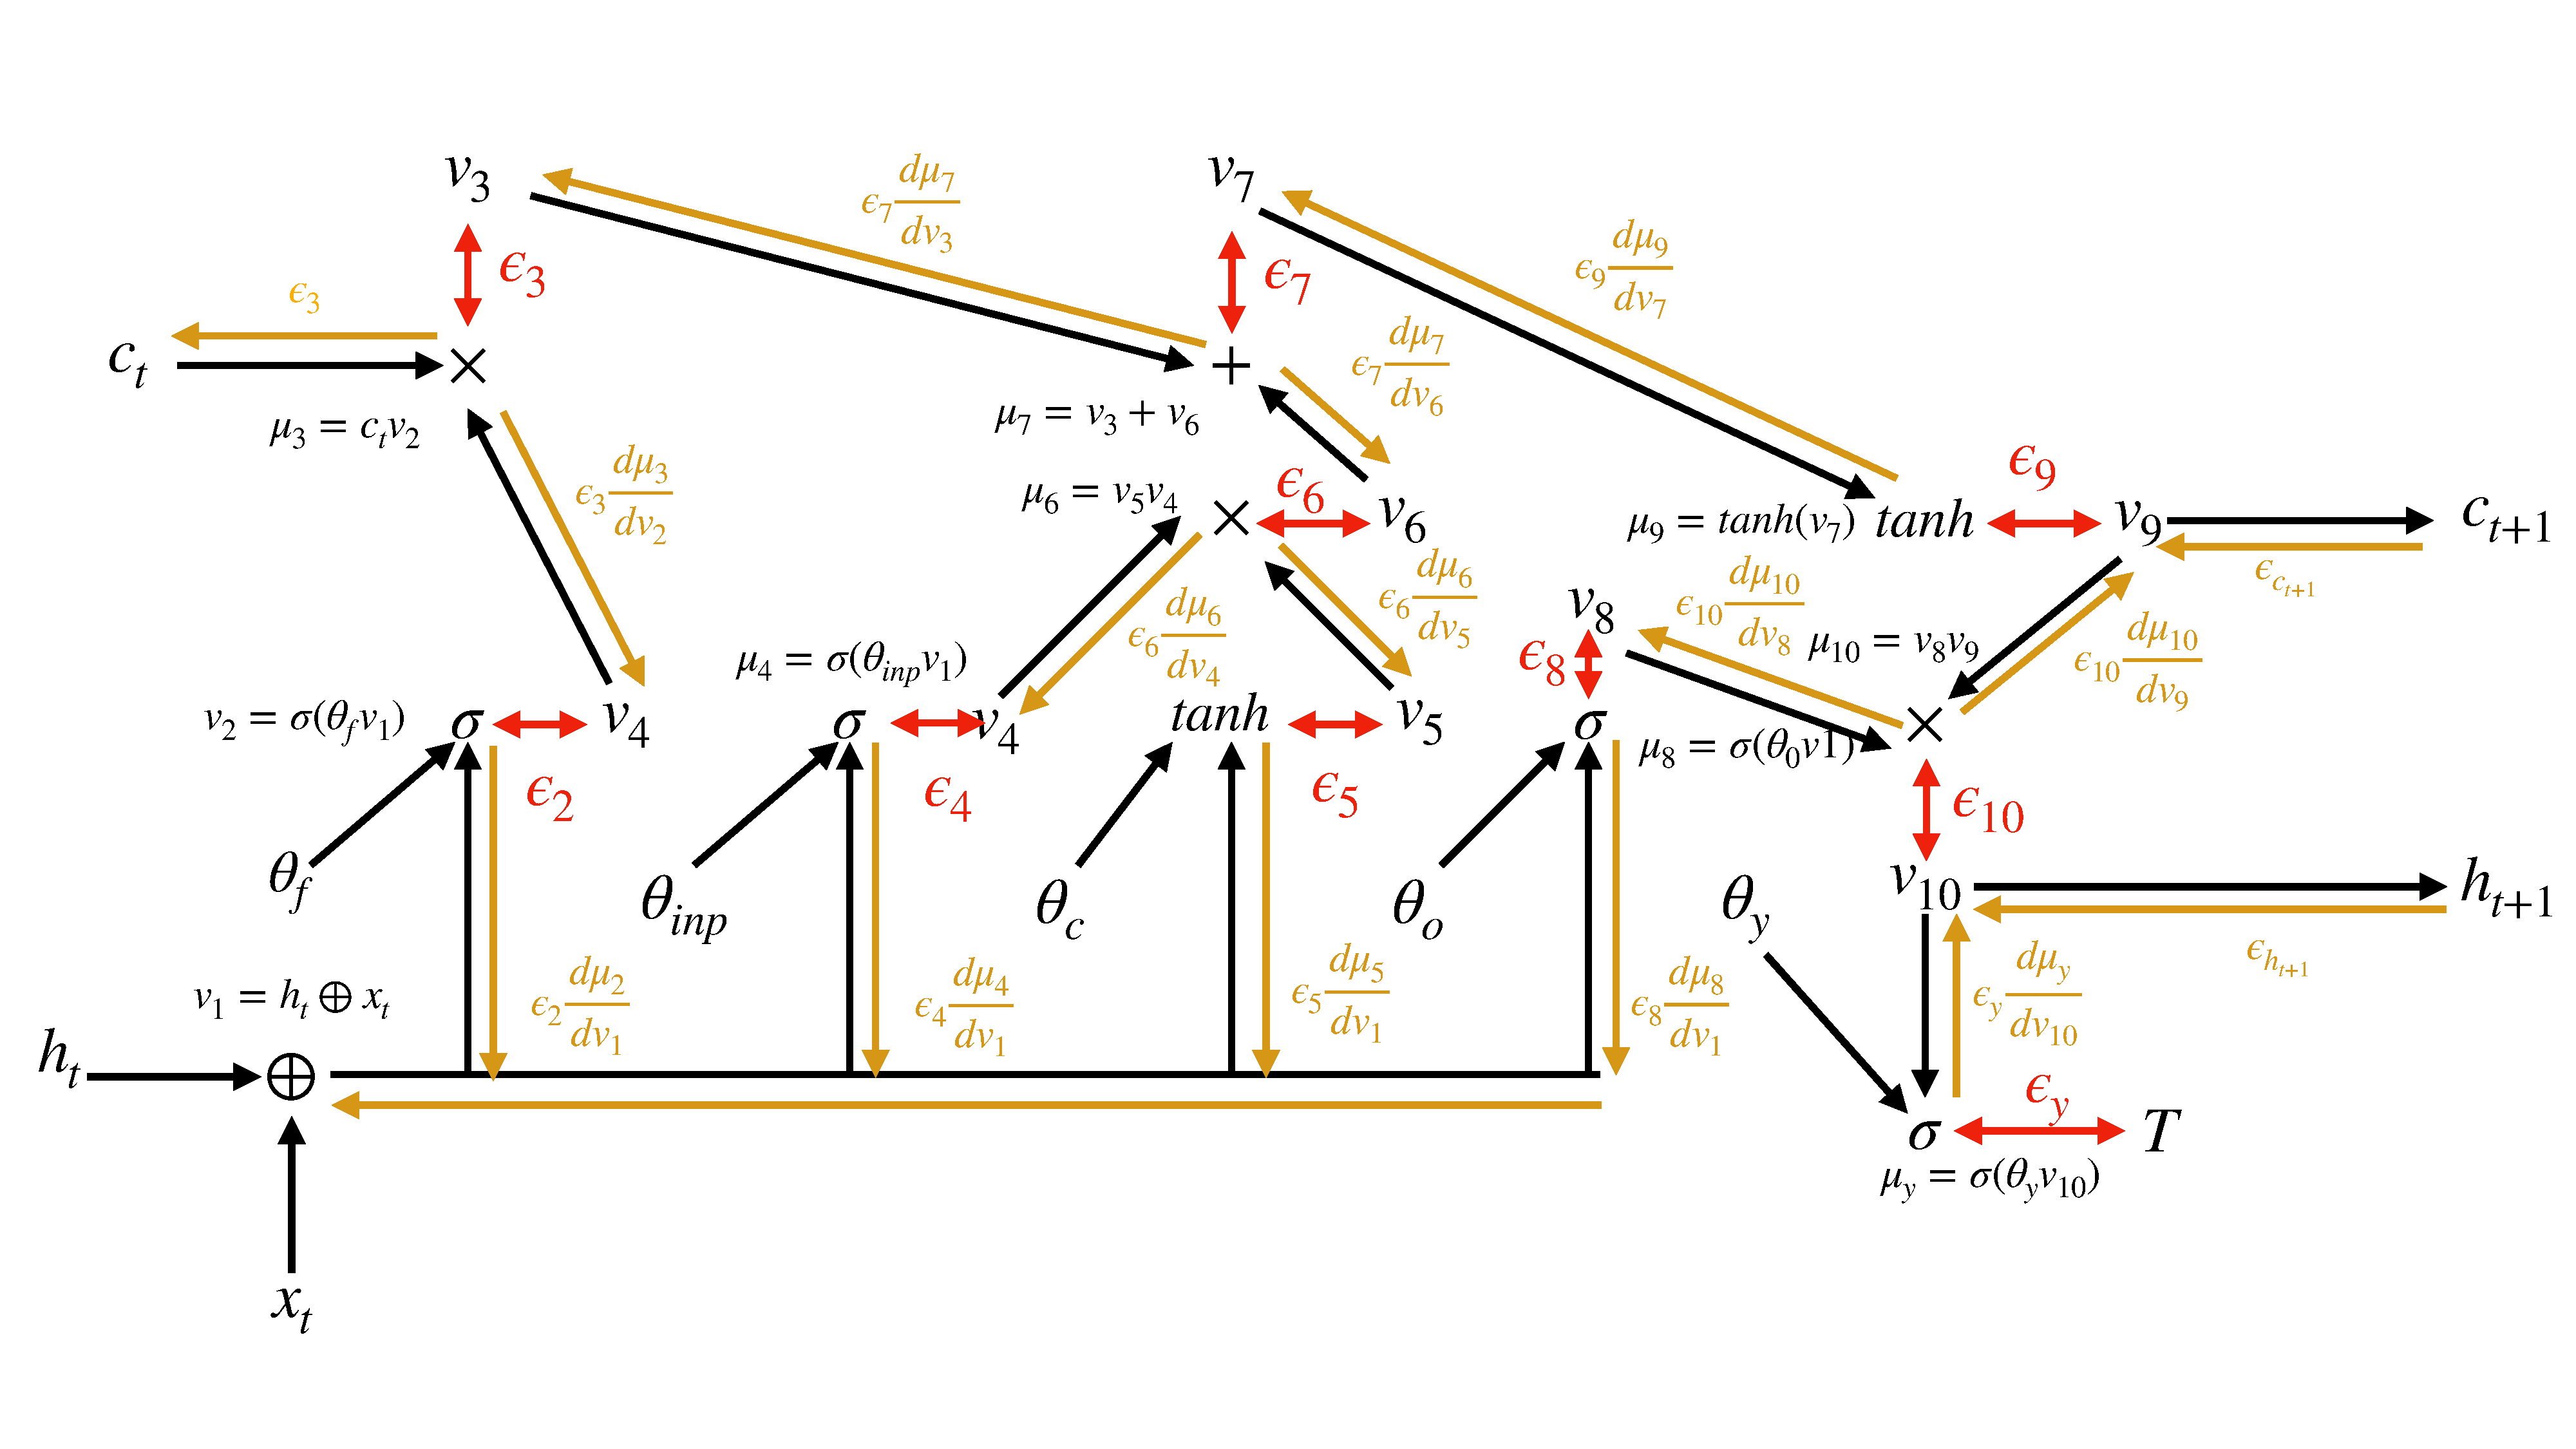
\includegraphics[width=1\linewidth]{chapter_6_figures/pc_LSTM.pdf}  
\caption{The LSTM cell computation graph augmented with error units, evincing the connectivity scheme of the predictive coding algorithm.}
\label{pc_lstm}
\end{figure}

For the LSTM we also observed a close correspondence between the performance (in terms of training and test accuracy) between the predictive coding and backpropagation networks, thus demonstrating that predictive coding can converge to the exact backprop gradients even on exceptionally deep and complex computation graphs such as the LSTM

\begin{figure}[ht]
  \centering
  % include first image
  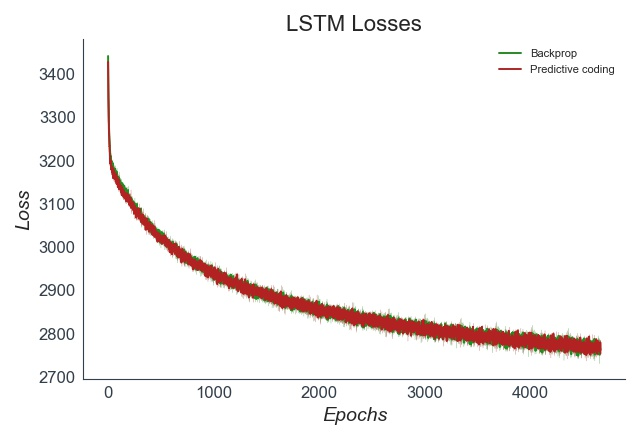
\includegraphics[width=0.7\linewidth]{chapter_6_figures/LSTM_Losses_super_prelim_6.jpg}  
\caption{Training losses for the predictive coding and backprop LSTMs averaged over 5 seeds. The performance of the two training methods is effectively equivalent.}
\label{LSTM_losses}
\end{figure}

Importantly, we observed rapid convergence to the exact backprop gradients even in the case of very deep computation graphs (as is an unrolled LSTM with a sequence length of 100). Although convergence was slower than was the case for CNNs or lesser sequence lengths, it was still straightforward to achieve convergence to the exact numerical gradients with sufficient iterations.

Below we plot the mean divergence between the predictive coding and true numerical gradients as a function of sequence length (and hence depth of graph) for a fixed computational budget of 200 iterations with an inference learning rate of 0.05. As can be seen, the divergence increases roughly linearly with sequence length. Importantly, even with long sequences, the divergence is not especially large, and can be decreased further by increasing the computational budget. As the increase is linear, we believe that predictive coding approaches should be scalable even for backpropagating through very deep and complex graphs.

We also plot the number of iterations required to reach a given convergence threshold (here taken to be 0.005) as a function of sequence length (Figure \ref{num_iterations_to_converge}). We see that the number of iterations required increases sublinearly with the sequence length, and likely asymptotes at about 300 iterations. Although this is a lot of iterations, the sublinear convergence nevertheless shows that the method can scale to even extremely deep graphs.

\begin{figure}[ht]
  \centering
  % include first image
  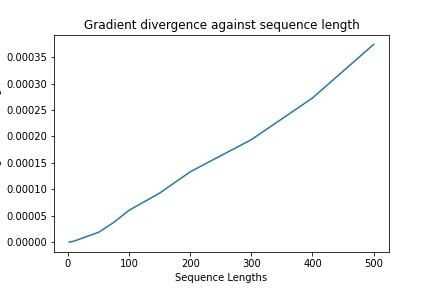
\includegraphics[width=.9\linewidth]{chapter_6_figures/lstm_seqlen_divergences.jpg}  
\caption{Divergence between predictive coding and numerical gradients as a function of sequence length.}
\label{sequence_length_effect}

\end{figure}

\begin{figure}[ht]
  \centering
  % include first image
  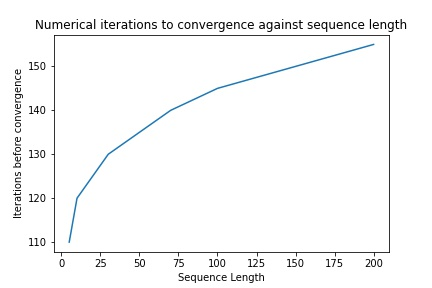
\includegraphics[width=.9\linewidth]{chapter_6_figures/convergence_num_iterations_comparison.jpg}  
\caption{Number of iterations to reach convergence threshold as a function of sequence length.}
\label{num_iterations_to_converge}
\end{figure}

Our architecture consisted of a single LSTM layer (more complex architectures would consist of multiple stacked LSTM layers).
The LSTM was trained on a next-character character-level prediction task. The dataset was the full works of Shakespeare, downloadable from Tensorflow. The text was shuffled and split into sequences of 50 characters, which were fed to the LSTM one character at a time. The LSTM was trained then to predict the next character, so as to ultimately be able to generate text. The characters were presented as one-hot-encoded vectors. The LSTM had a hidden size and a cell-size of 1056 units. A minibatch size of 64 was used and a weight learning rate of 0.0001 was used for both predictive coding and backprop networks. To achieve sufficient numerical convergence to the correct gradient, we used 200 variational iterations with an inference learning rate of 0.1. This rendered the predictive LSTM approximately 200x as costly as the backprop LSTM to run. A graph of the LSTM training loss for both predictive coding and backprop LSTMs, averaged over 5 random seeds, can be found below (Figure \ref{pcbp_lstm_losses}). 

\begin{figure}[ht]
  \centering
  % include first image
  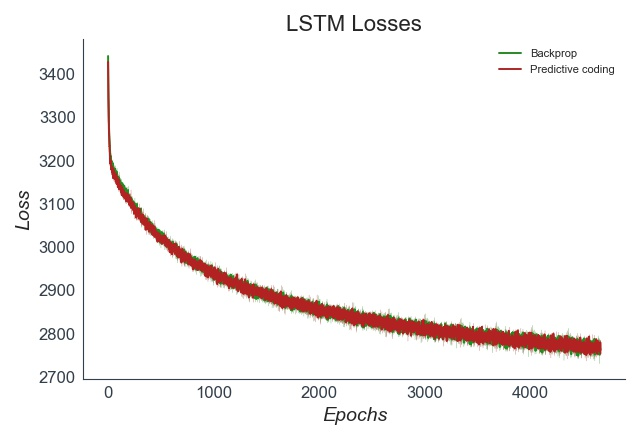
\includegraphics[width=0.7\linewidth]{chapter_6_figures/LSTM_Losses_super_prelim_6.jpg}  
\caption{Training losses for the predictive coding and backprop LSTMs averaged over 5 seeds. The performance of the two training methods is effectively equivalent.}
\label{pcbp_lstm_losses}
\end{figure}

\section{Interim Discussion}

Here we have shown that predictive coding can be applied directly to arbitrary computation graphs and can rapidly and effectively converge to the exact gradients required for the backpropagation of error algorithm. We have demonstrated this on deep and state of the art machine learning architectures, thus achieving significantly greater scale than previous works using predictive coding \citep{millidge2019implementing,orchard2019making,whittington2017approximation}. Moreover, the predictive coding learning rule uses only local learning dynamics and Hebbian weight updates in the case of the usual feedforward neural networks (although they differ somewhat for the LSTM). Weights are updated using only local prediction errors. 

This approach also is innovative in that it phrases backprop in terms of variational inference on the values of the nodes in the computation graph. While it may seem just like a mathematical convenience, it actually has deep implication. It draws another link between the processes of optimization and variational inference, in a rather different manner from that which has largely been explored before. Instead of conceptualising inference as optimization, as is typically done in variational inference, we instead conceptualize a core component of optimization -- credit assignment -- purely in terms of inference. While this duality has been considered before for two layer networks \citep{amari1995information}, our approach is substantially more powerful and general, by showcasing that it holds for arbitrary computation graphs. Additionally, our approach provides an avenue for interesting generalizations of backprop through the use of precision parameters in predictive coding. Note that in our analysis, we have implicitly assumed that all of the precision parameters are set to the identity $\Sigma = \mathbb{I}$, as they do not feature in the learning and update rules, as they do in Chapter 3. If we reintroduce precision in this context, we see that it has the role of modulating gradient magnitudes -- effectively implementing an adaptive learning rate. What this means, intuitively, is that we can think about precision weighting in this case as enabling an \emph{uncertainty aware backprop}, which specifically weights gradients by how uncertain they are -- or by their variance. Effectively, this method, with learnable precisions, would down-weight highly variable and uncertain gradients while upweighting those known to be certain. When applied to the input this would mimic features of attention, by downweighting noisy or otherwise uncertain inputs and having them play little role in learning. While such an adaptive modulatory role for precision may bring learning benefits, this must be explored further, as the author hopes to do in future work.

Finally, it is worth discussing several drawbacks of the method. The key one is its computational cost. The networks presented here were trained with 100 dynamical iterations to converge to the prediction error equilibrium before each weight update, giving predictive coding an approximately 100x computational cost compared to backprop. This is obviously highly significant and renders these approaches unusable for large scale networks on serial Von-Neumann computers. While the brain utilizes highly parallel circuitry, and may therefore be more suited to such an iterative algorithm, there are still issues with requiring a dynamical iteration for convergence. Specifically, such iterations still require time and discrete phases so that the system cannot likely simply operate in continuous time. Moreover, if too many iterations are required, since the brain must respond to a continually changing world instead of just single images presented in isolation, it may become overwhelmed by events and fail computationally, if the input changes faster than it can dynamically converge to a solution. While not necessarily as severe as needing dynamical approaches for \emph{inference}, which would entirely hamstring any response, here the dynamics are only required for learning and weight updates, this may nevertheless prove to be a substantial drawback of the method. Our method, like most others, also requires two distinct phases which must either be somehow coordinated explicitly, or multiplexed in the brain.

Additionally, the fixed-prediction assumption embedded in the model requires maintaining the stored memory of the feedforward pass values somewhere in the network throughout the backwards dynamical phase which is potentially problematic in neural circuitry. Finally, although the predictive coding learning rules are local, in the sense that they only require information from the same layer, they still require information from the prediction error units to be transmitted to the activity units, where we assume the synaptic weights are located (although in a segregated dendrite model they could just be in different dendrites \citep{sacramento2018dendritic}).

\section{Activation Relaxation}
% rationalize notation with intro
Here we introduce a second iterative algorithm which approximates the exact backpropagation gradients asymptotically at the equilibrium of a dyanamical system. We call this algorithm \emph{Activation Relaxation} (AR) because of the nature of the update rules, which iteratively update the \emph{activations} of neurons in the iterative phase rather than prediction errors. Crucially, the update rules proposed by AR are exceedingly simple and elegant, and do not require additional populations of `error neurons' as in predictive coding, or multiple backwards phases as in Equilibirium-prop. AR arises quite straightforwardly by trying to take a first principles approach to the iterative backprop approximation schemes.

To establish notation, we consider the simple case of a fully-connected deep multi-layer perceptron (MLP) composed of $L$ layers of rate-coded neurons trained in a supervised setting. The firing rates of these neurons are represented as a single scalar value $x^l_i$, referred to as the neurons activation,  and a vector of all activations at given layer is denoted as $x^l$. The activations of the hierarchically superordinate layer are a function of the hierarchically subordinate layers activations $x^{l+1} = f(W^l x^l)$, where $W^l \in \Theta$ is the set of synaptic weights, and the product of activation and weights is transformed through a nonlinear activation function $f$. The final output $x^L$ of the network is compared with the desired targets $T$, according to some loss function $\mathcal{L}(x^L, T)$. In this work, we take this loss function to be the mean-squared-error (MSE) $\mathcal{L}(x^L, T) = \frac{1}{2}\sum_i (x^L_i - T_i)^2$, although the algorithm applies to any other loss function without loss of generality (see Appendix B). We denote the gradient of the loss with respect to the output layer as $\frac{dL}{dx^L}$. In the case of the MSE loss, the gradient of the output layer is just the prediction error $\epsilon^L = (x^L - T)$.

Firstly, we know that the key quantity we wish to approximate is the adjoint term $\frac{\partial \mathcal{L}}{\partial x_l}$ for a given layer $l$. If we know this adjoint, and have it present somewhere in the local environment, then the gradient with respect to the weights can be computed using only locally available information. In predictive coding, we compute this adjoint term using the recursive relationship of the prediction errors. Here, we take a different approach. Instead, we ask  what is the simplest possible dynamical system which can converge to the exact adjoint term at the equilibrium. After some thought, we emerge at a straightforward leaky integrator model.
\begin{align*}
\label{AR_initial_equation}
    \frac{d x^l}{dt} &= -x^l + \frac{\partial \mathcal{L}}{\partial x^l} \numberthis 
 \end{align*}
    which, at equilibrium, converges to \vspace{-0.2cm}
\begin{align*}
\label{AR_equilibrium_equation}
     \frac{dx^l}{dt} =0 &\implies {x^*}^l = \frac{\partial \mathcal{L}}{\partial x^l} \numberthis
\end{align*}

This update rule includes the very adjoint term we are trying to compute, however, so these dynamics are not immediately computable. To make them so, we first split up the adjoint using the chain rule to obtain,
Furthermore, by the chain rule we can write Equation \ref{AR_initial_equation} as,
\begin{align*}
    \frac{dx^l}{dt} = -x^l + \frac{\partial \mathcal{L}}{\partial x^{l+1}}\frac{\partial x^{l+1}}{\partial x^l} \Bigr|_{x^l=\bar{x}^l} \numberthis
\end{align*}
where $\bar{x}^l$ is the value of $x^l$ computed in the forward pass. Next, we note that if we use the \emph{activations of the neurons at each layer} instead of prediction errors to accumulate the adjoint, we can express this in terms of the equilibrium activation of the superordinate layer,
    \begin{align*}
    \frac{dx^l}{dt} =  -x^l + {x^*}^{l+1} \frac{\partial x^{l+1}}{\partial x^l} \Bigr|_{x^l=\bar{x}^l} \numberthis
\end{align*}
However, to achieve these dynamics exactly in a multilayered network would require the sequential convergence of layers, as each layer must converge to equilibrium before the dynamics of the layer below can operate. This sequential convergence would make the algorithm no better than the sequential backwards sweep of backprop. However, if we approximate the equilibrium activations of the layer with the current activation, this allows us to run all layers in parallel, yielding,
\begin{align*}
\label{AR_main_equation}
    \frac{dx^l}{dt} &=  -x^l + {x^*}^{l+1} \frac{\partial x^{l+1}}{\partial x^l}\Bigr|_{x^l=\bar{x}^l} \\
    &\approx -x^l + x^{l+1}\frac{\partial x^{l+1}}{\partial x^l} \Bigr|_{x^l=\bar{x}^l} \numberthis \\
    &\approx -x^l + x^{l+1}f'(W^l, \bar{x}^l) {W^l}^T  \numberthis
\end{align*}
where $f' = \frac{\partial f'(W^l, \bar{x}^l)}{\partial \bar{x}^l}$ represents the partial derivative of the postsynaptic activation with respect to the presynaptic activation. Despite this approximation, we argue that the system nevertheless converges to the same optimum as Equation \ref{AR_equilibrium_equation}. Specifically, because we evaluate $\frac{\partial x^{l+1}}{\partial x^l}$ at the feedforward pass value $\bar{x}^l$, this term remains constant throughout the relaxation phase \footnote{The need to keep this term fixed throughout the relaxation phase does present a potential issue of biological plausibility. In theory it could be maintained by short-term synaptic traces, and for some activation functions such as rectified linear units it is trivial. Moreover, later we show that this term can be dropped from the equations without apparent ill-effect}. Keeping this term fixed effectively decouples the each layer from any bottom-up influence. If the top-down input is also constant, because it has already converged so that $x^{l+1} \approx {x^{l+1}}^*$, then the dynamics become linear, and the system is globally stable due to possessing a Jacobian which is everywhere negative-definite. The top-layer is provided with the stipulatively correct gradient, so it must converge. Recursing backwards through each layer, we see that once the top-level has converged, so too must the penultimate layer, and so through to all layers.

Crucially, Equation \ref{AR_main_equation}, which is core to the AR algorithm is extremely simple and biologically plausible. It only requires that the activations of a given layer are sensitive to the difference between their own activity and that of the layer above mapped through the backwards weights, and modulated by the nonlinear derivative of the postsynaptic potential. This update rule thus functions as a kind of prediction error, but one that emerges between layers, rather than being represented by specific prediction error units at a given layer.

Computationally, the AR algorithm proceeds as follows. First, a standard forward pass computes the network output, which is compared with the target to calculate the top-layer error derivative $\epsilon_L$ and thus update the activation of the penultimate layer. \footnote{This top-layer error is simply a prediction error for the MSE loss, but may be more complicated and less biologically-plausible for arbitrary loss functions}. Then, the network enters into a relaxation phase where Equation \ref{AR_main_equation} is iterated globally for all layers until convergence for each layer. 
Upon convergence, the activations of each layer are precisely equal the backpropagated derivatives, and are used to update the weights (via Equation (\ref{BP_weights_equation}).
\begin{align*}
\label{BP_weights_equation}
    \frac{\partial L}{\partial W^l} &= \frac{\partial L}{\partial x^{l+1}}\frac{\partial x^{l+1}}{\partial W^l} \\
    &= \frac{\partial L}{\partial x^{l+1}}f'(W^l x^l) {x^L}^T \numberthis
\end{align*}
\newline
\begin{algorithm}[H]
\DontPrintSemicolon
\SetAlgoLined
\textbf{Dataset} $\mathcal{D} = \{\mathbf{X},\mathbf{T}\}$, parameters $\Theta = \{W^0 \dots W^L\}$, inference learning rate $\eta_x$, weight learning rate $\eta_\theta$.
\BlankLine
%\tcc{Iterate over dataset}
\For{$(x^0, t \in \mathcal{D})$}{
    %\tcc{Initial feedforward sweep} 
    \For{$(x^l,W^l)$ for each layer}{
        $x^{l+1} = f(W^l, x^l)$ 
    }
    %\tcc{Begin backwards relaxation}
    \While{not converged}{
        %\tcc{Compute final output error} 
        $\epsilon^L = T - x^L $ \\ 
        $ dx^L= -x^L +  \epsilon^L \frac{\partial \epsilon^L}{\partial x^L} $ \\
        \For{$x^l, W^l, x^{l+1}$ for each layer}{
        %\tcc{Activation update} 
         $dx^l = -x^l +  x^{l+1} \frac{\partial x^{l+1} }{\partial x^l}$ \\
        ${x^l}^{t+1} \leftarrow {x^l}^t + \eta_x dx^l $
        }
    }
    %\tcc{Update weights at equilibrium}
    \For{$W^l \in \{W^0 \dots W^L \}$}{
        ${W^l}^{t+1} \leftarrow {W^l}^t + \eta_\theta x^l \frac{\partial x^l}{\partial W^l}$ 
    }
    }
\caption{Activation Relaxation}
\end{algorithm} 

\section{Method and Results}

We first demonstrate that our algorithm can train a deep neural network with equal performance to backprop. For training, we utilised the MNIST and Fashion-MNIST \citep{xiao2017online} datasets. The MNIST dataset consists of 60000 training and 10000 test 28x28 images of handwritten digits, while the Fashion-MNIST dataset consists of 60000 training and 10000 test 28x28 images of clothing items. The Fashion-MNIST dataset is designed to be identical in shape and size to MNIST while being harder to solve. We used a 4-layer fully-connected multi-layer perceptron (MLP) with rectified-linear activation functions and a linear output layer. The layers consisted of 300, 300, 100, and 10 neurons respectively. In the dynamical relaxation phase, we integrate  Equation \ref{AR_main_equation} with a simple first-order Euler integration scheme. ${x^l}^{t+1} = {x^l}^t - \eta_x \frac{dx^l}{dt}$ where $\eta_x$ was a learning rate which was set to $0.1$. The relaxation phase lasted for 100 iterations, which we found sufficient to  closely approximate the numerical backprop gradients. After the relaxation phase was complete, the weights were updated using the standard stochastic gradient descent opteimizer, with a learning rate of 0.0005. The weights were initialized as draws from a Gaussian distribution with a mean of 0 and a variance of 0.05.  Hyperparameter values were chosen based off initial intuition and were not found using a grid-search. 
The AR algorithm was applied to each minibatch of 64 digits sequentially. The network was trained with the mean-squared-error loss.
\begin{figure}
\centering
\subfloat[MNIST train accuracy]{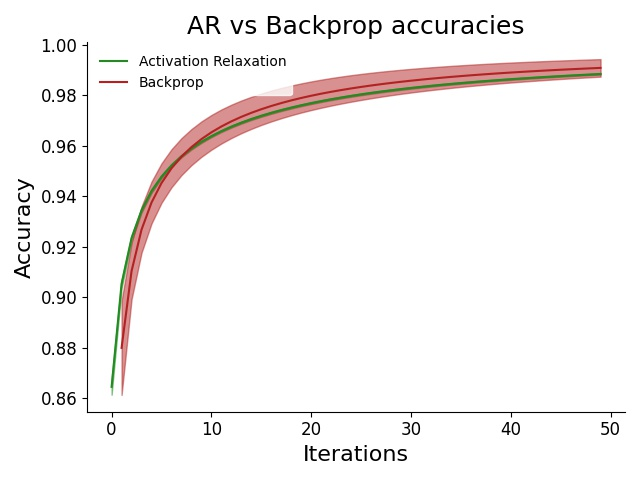
\includegraphics[width=0.3\linewidth]{chapter_6_figures/AR/mnist_AR_vs_Backprop_accuracies.jpg}}\hfil
\subfloat[MNIST test accuracy]{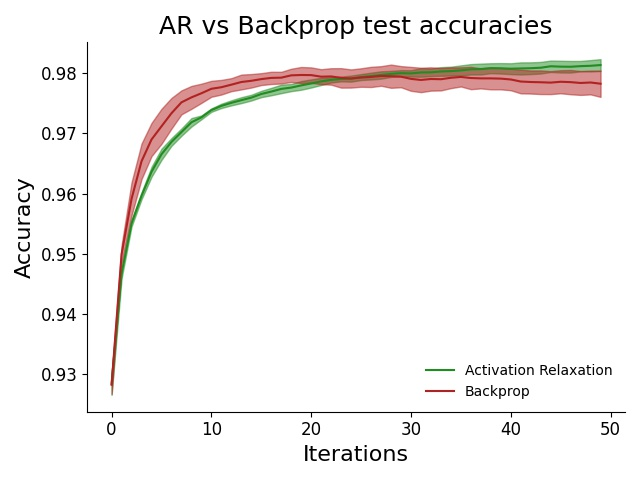
\includegraphics[width=0.3\linewidth]{chapter_6_figures/AR/mnist_AR_vs_Backprop_test accuracies.jpg}}\hfil 
\subfloat[MNIST gradient angle]{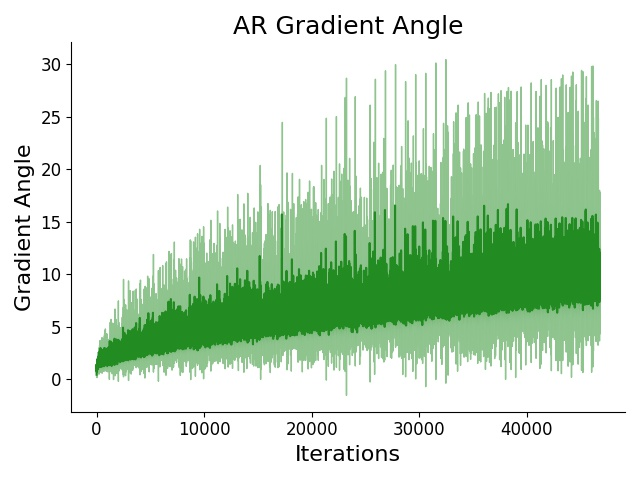
\includegraphics[width=0.3\linewidth]{chapter_6_figures/AR/mnist_AR_Gradient_Angle_grad_angle.jpg}} 

\subfloat[Fashion train accuracy]{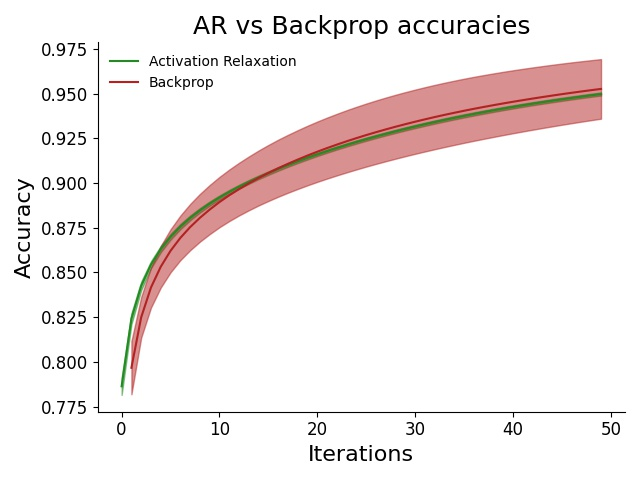
\includegraphics[width=0.3\linewidth]{chapter_6_figures/AR/fashion_AR_vs_Backprop_accuracies.jpg}}\hfil
\subfloat[Fashion test accuracy]{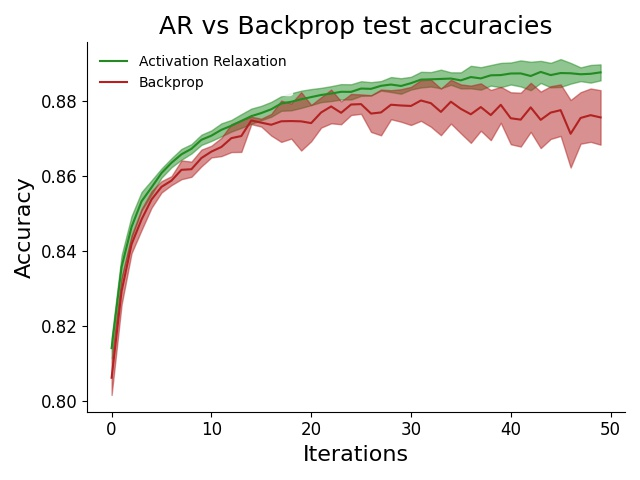
\includegraphics[width=0.3\linewidth]{chapter_6_figures/AR/fashion_AR_vs_Backprop_test accuracies.jpg}}\hfil AR/
\subfloat[Fashion gradient angle]{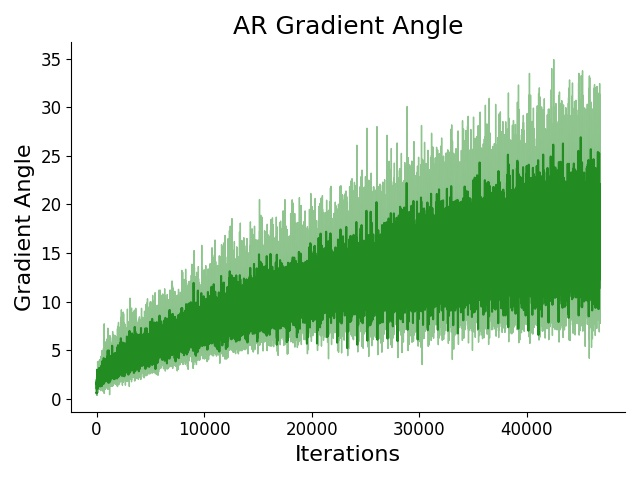
\includegraphics[width=0.3\linewidth]{chapter_6_figures/AR/fashion_AR_Gradient_Angle_grad_angle.jpg}}
\caption{Train and test accuracy and gradient angle (cosine similarity) for AR vs backprop for MNIST and Fashion-MNIST datasets.}
\label{AR_mnist_results}
\end{figure}

In Figure \ref{AR_mnist_results} we show that the training and test performance of the network trained with activation-relaxation is nearly identical to that of the network trained with backpropagation, thus demonstrating that our algorithm can correctly perform credit assignment in deep neural networks with only local learning rules. We also empirically investigate the angle between the AR-computed gradient updates and the true backpropagated updates. The gradient angle $\mathcal{A}$ was computed using the cosine similarity metric $\mathcal{A}(\nabla_\theta) =  \cos^{-1} \frac{\nabla_\theta^T \nabla_\theta^*}{||\nabla_\theta|| ||\nabla_\theta^*}$, where $\nabla_\theta$ was the AR-computed gradients and $\nabla_\theta^*$ were the backprop gradients. To handle the fact that we had gradient matrices while the cosine similarity metric only applies to vectors, following \citep{lillicrap2016random}, we simply flattened the gradient matrices into vectors before performing the computation. We see that the updates computed by AR are very close in angle to the backprop updates (within under 10 degrees), although the angle increases slightly over the course of training. The convergence in training and test accuracies between the AR and backprop shows that this slight difference in gradient angle is not enough to impede effective credit assignment and learning in AR. In Appendix C, we take a step towards demonstrating the scalability of this algorithm, by showing preliminary results that indicate that AR, including with the biologically plausible simplifications introduced below, can scale to deeper CNN architectures and more challenging classification tasks.

\subsection{Loosening Constraints}

While the AR algorithm as above precisely approximates adjoint term $\frac{\partial \mathcal{L}}{\partial x^l}$ central to backprop, using only local learning rules, it still retains a number of biological implausibilities. The core implausibility is the weight transport problem, which is still present due to the weight transpose present in Equation \ref{AR_main_equation}.  Following our previous work on relaxed predictive coding (Chapter 3), we demonstrate how the same remedies can be directly applied to the AR algorithm without jeopardising learning performance.

To address the weight transport problem, we take inspirations from the approaches of feedback alignment \citep{lillicrap2016random}, and \citep{millidge2020relaxing}. We postulate an independent separate set of backwards weights $\psi^l$, so that the update rule for the activations becomes,
\begin{align*}
    \frac{dx^l}{dt} = x^l - x^{l+1}f'(W^l x^l) \psi^l \numberthis
\end{align*} 
Then, following our work on relaxed preditive coding in Chapter 5, we learn these backwards weights with the following Hebbian update,
\begin{align*}
\label{AR_psi_equation}
    \frac{d\psi^l}{dt} = {x^{l+1}}^T f'(W^l x^l) x^l \numberthis
\end{align*}

The backwards weights were initialized as draws from a 0 mean, 0.05 variance Gaussian. In Figure \ref{AR_results_figures} we show that strong performance is obtained with the learnt backwards weights. We found that using random feedback weights without learning (i.e. feedback alignment), typically converged to a lower accuracy and had a tendency to diverge, which may be due to a simple Gaussian weight initialization used here. Nevertheless, when the backwards weights are learnt, we find that the algorithm is stable and can obtain performance comparable with using the exact weight transposes (Figure \ref{AR_results_figures}).  This is a very strong and encouraging result. First that this learning rule enables performance with exact weight transposes is impressive, since it implies that the Hebbian update rule on the backwards weights works and is highly effective, even early on in training. Secondly, the generalizability of this remedy for weight transport, from predictive coding networks, deep neural networks \citep{amit2019deep,akrout2019deep} with backprop, and now AR suggests that the backwards weights may be able to be independent and robustly learned from scratch in the brain, thus largely resolving the weight transport problem altogether.

\begin{figure}
\centering
\subfloat[MNIST backwards weights]{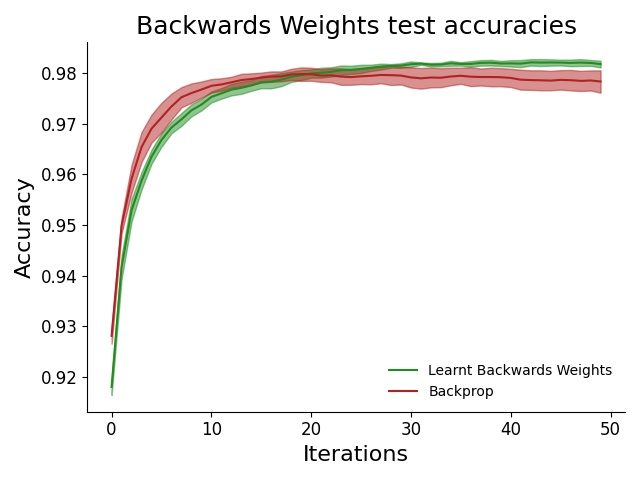
\includegraphics[width=0.3\linewidth]{chapter_6_figures/AR/mnist_Backwards_Weights_test accuracies.jpg}}\hfil
\subfloat[MNIST nonlinear derivatives]{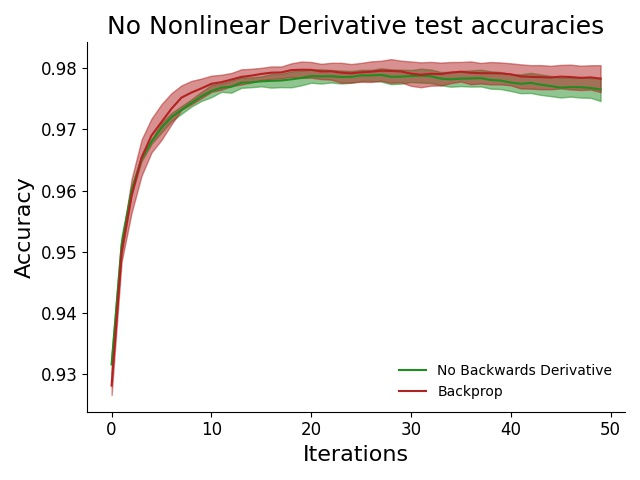
\includegraphics[width=0.3\linewidth]{chapter_6_figures/AR/mnist_No_Nonlinear_Derivative_test accuracies.jpg}}\hfil 
\subfloat[MNIST combined]{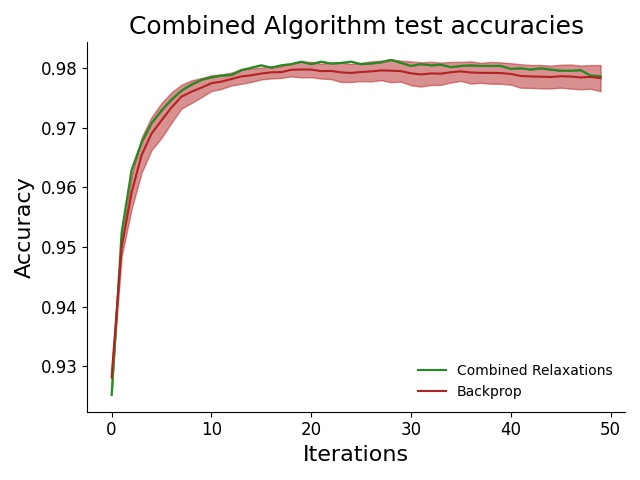
\includegraphics[width=0.3\linewidth]{chapter_6_figures/AR/mnist_Combined_Algorithm_test accuracies.jpg}} 

\subfloat[Fashion backwards weights]{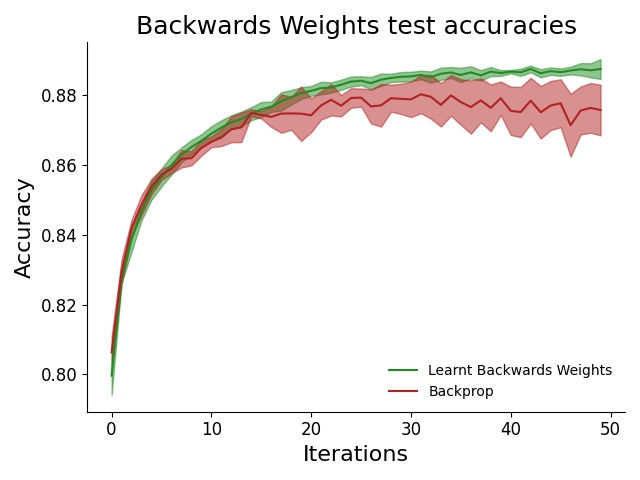
\includegraphics[width=0.3\linewidth]{chapter_6_figures/AR/fashion_Backwards_Weights_test accuracies.jpg}}\hfil
\subfloat[Fashion nonlinear derivatives]{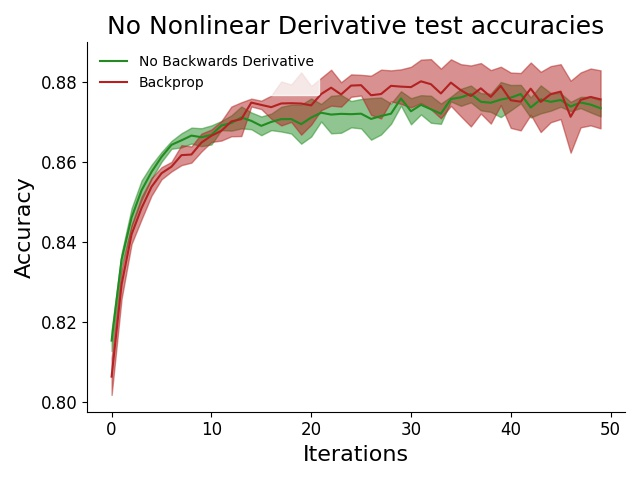
\includegraphics[width=0.3\linewidth]{chapter_6_figures/AR/fashion_No_Nonlinear_Derivative_test accuracies.jpg}}\hfil 
\subfloat[Fashion combined]{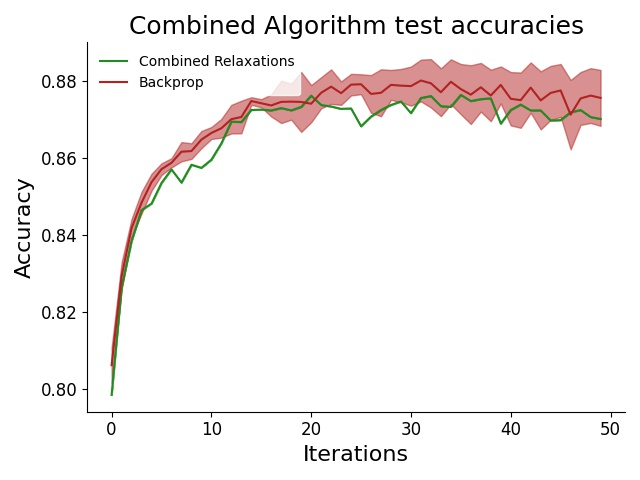
\includegraphics[width=0.3\linewidth]{chapter_6_figures/AR/fashion_Combined_Algorithm_test accuracies.jpg}} 
\caption{Train and test accuracy and gradient angle (cosine similarity) for AR vs backprop for MNIST and Fashion-MNIST datasets.}
\label{AR_results_figures}
\end{figure}

We additionally  plot the angle between the AR with learnable backwards weights and the true BP gradients (Figure \ref{AR_grad_angle_figure}). The angle starts out very large (about 70 degrees) since the backwards weights are randomly initialized but then rapidly decreases to about 30 degrees as the backwards weights are learnt, which seems empirically to be sufficient to enable strong learning performance. 

An additional potential biological implausibility to address is the nonlinear derivative problem, which consists of the $f'(W^l, \bar{x}^l) {W^l}^T$ term. The biological plausibility of this term depends heavily upon the activation function used in the network. For instance, in a relu network, this term is trivial, being 0 if the postsynaptic output is greater than 0, and 1 if it is. However, other commonly used activation functions like tanh, sigmoid, and especially softmax are more complex and may be challenging to compute locally in the brain. Here, we experiment with simply dropping the nonlinear derivative term from the update rule, which results in the following dynamics,

\begin{align*}
\frac{dx^l}{dt} = x^l - x^{l+1}{W^l}^T \numberthis
\end{align*}
Although the gradients are no longer match backprop, we show in Figure \ref{AR_results_figures} that learning performance against the standard model is relatively unaffected, showing that the influence of the nonlinear derivative is small. We hypothesise that by removing the nonlinear derivative, we are effectively projecting the backprop update onto the closest linear subspace, which is still sufficiently close in angle to the true gradient that it can support learning. Alternatively, it could be that in the regime of standard activity values prevailing throughout the network during training, the nonlinear derivatives generally are close to 1, and thus have little effect on the update rules in any case. If this is the case, then given that we made no particular effort to constrain the activities of the network, it supposes that this property, if it exists, may be highly beneficial for simplifying the computations in the brain.

By explicitly plotting the angle (Figure \ref{AR_grad_angle_figure}), we see that it always remains under about 30 degrees, sufficient for learning, although the angle appears to rise over the course of training, potentially due to the gradients becoming smaller and more noisy as the network gets closer to convergence.


\begin{figure}
% relaxations gradient angle graph
\centering
\subfloat[Backwards weight angle]{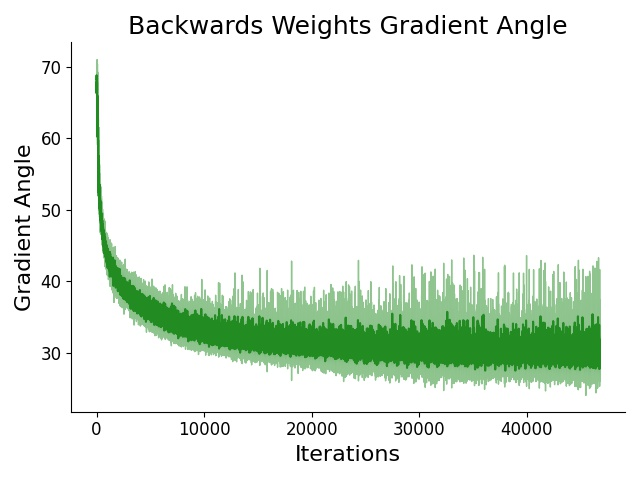
\includegraphics[width=0.3\linewidth]{chapter_6_figures/AR/mnist_Backwards_Weights_Gradient_Angle_grad_angle.jpg}}\hfil
\subfloat[Nonlinear derivatives angle]{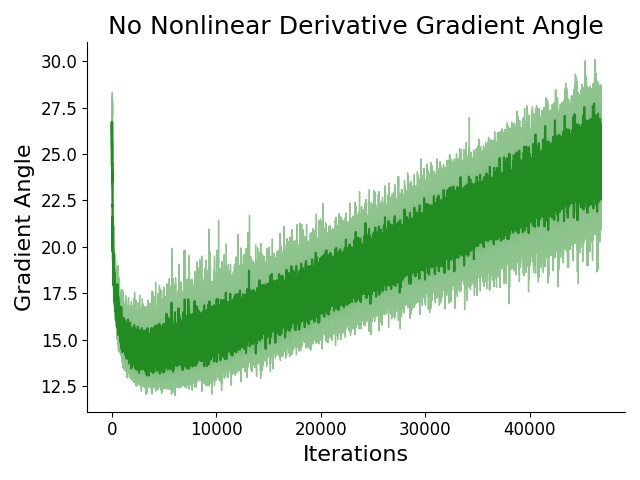
\includegraphics[width=0.3\linewidth]{chapter_6_figures/AR/mnist_No_Nonlinear_Derivative_Gradient_Angle_grad_angle.jpg}}\hfil 
\subfloat[Combined angls]{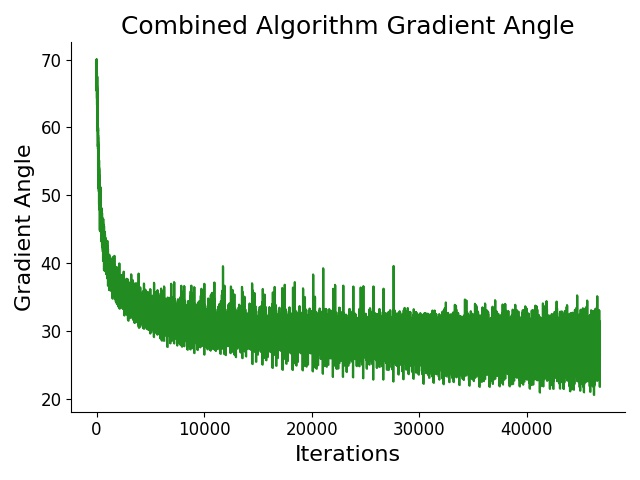
\includegraphics[width=0.3\linewidth]{chapter_6_figures/AR/mnist_Combined_Algorithm_Gradient_Angle_grad_angle.jpg}} 
\caption{Angle between the AR and backprop updates in the learnable backwards weights, no nonlinear derivatives, and the combined conditions.}
\label{AR_grad_angle_figure}
\end{figure}

Moreover, we can \emph{combine} these two changes of the algorithm such that there is both no nonlinear derivative and also learnable backwards weights. Perhaps surprisingly, when we do this  we retain equivalent performance to the full AR algorithm (see Figure \ref{AR_results_figures}), and therefore a valid approximation to backprop in an extremely simple and biologically plausible form. The activation update equation for the fully simplified algorithm is: 
\vspace{-0.2cm}
\begin{align*}
\label{fully_relaxed_AR_update}
    \frac{dx^l}{dt} = x^l - x^{l+1}\psi \numberthis
\end{align*}
which requires only locally available information and is mathematically very simple. In effect, each layer is only updated using its own activations and the activations of the layer above mapped backwards through the feedback connections, which are themselves learned through a local and Hebbian learning rule. This rule maintains high training performance and a close angle between its updates and the true backprop updates (Figure \ref{AR_grad_angle_figure}), and is, at least in theory, relatively straightforward to implement in neural or neuromorphic circuitry.

Finally, we note that the AR update rules require the nonlinear derivative $f'(W^l x^l)$ to be evaluated with the activity $x^l$ evaluated at its feedforward pass value $x^l = \bar{x}^l$. Additionally, in the weight update, the value of the activity $x^l$ needs to be evaluated at its feedforward pass value
\begin{align*}
    \frac{\partial \mathcal{L}}{\partial W^l} = \frac{\partial \mathcal{L}}{\partial x^{l+1}}\frac{\partial x^{l+1}}{\partial W^l} \Bigr|_{x^{l+1}=\bar{x}^{l+1}}  = {x^{l+1}}^* \bar{x}^T {\frac{\partial f(W^l \bar{x}^l)}{\partial \bar{x}}}^T \numberthis
\end{align*}
We call this the \emph{frozen feedforward pass} assumption, and it is very closely related to the fixed-prediction assumption in predictive coding or, similarly the requirement in equilibrium-propagation to store all the intermediate equilibrium values of the free phase. Here we investigate to what extent this assumption can also be relaxed. 

We evaluate whether the nonlinear derivative term can be unfrozen so that it uses the current value of the activity in a.) the function derivative $f'$ in Equation \ref{AR_main_equation}, b.) in the weight update equation (Equation \ref{BP_weights_equation}), and c.) we investigate whether the activation value itself can be replaced in the weight update equation.
\begin{figure}[htb]
\centering
  \begin{subfigure}[b]{0.4\linewidth}
    \centering
    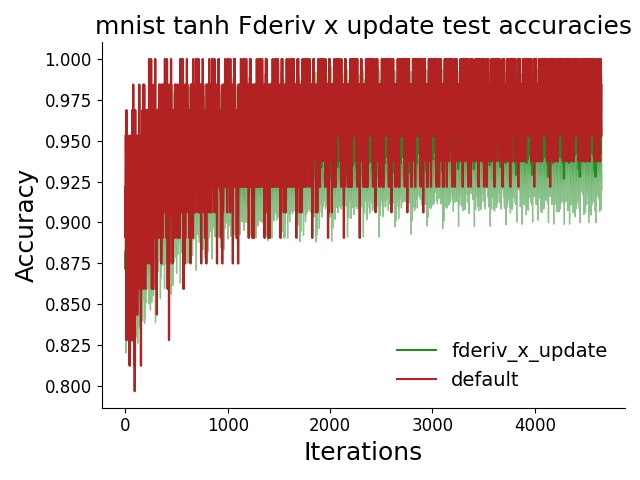
\includegraphics[width=0.75\linewidth]{chapter_6_figures/AR/mnist_tanh_Fderiv_x_update_test_accuracies_prelim_2.jpg} 
    \caption{MNIST nonlinear derivative relaxation update} 
    \vspace{4ex}
  \end{subfigure}%% 
  \begin{subfigure}[b]{0.4\linewidth}
    \centering
    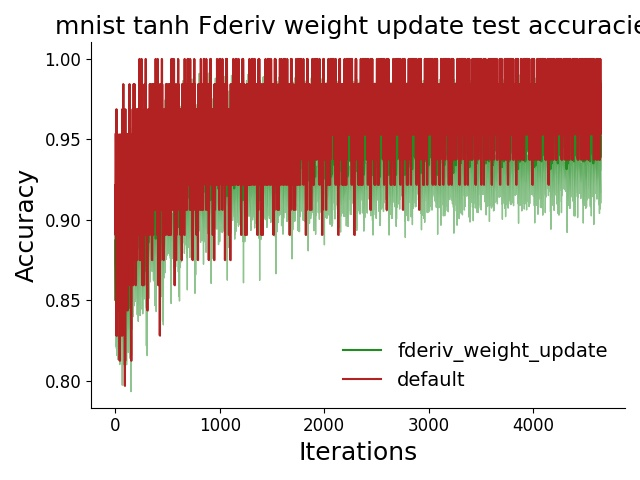
\includegraphics[width=0.75\linewidth]{chapter_6_figures/AR/mnist_tanh_Fderiv_weight_update_test_accuracies_prelim_2.jpg} 
    \caption{MNIST nonlinear derivative weight update} 
    \vspace{4ex}
  \end{subfigure} 
  \begin{subfigure}[b]{0.4\linewidth}
    \centering
    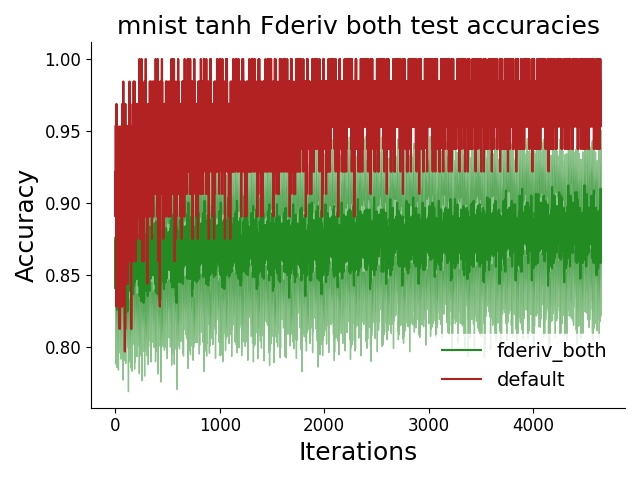
\includegraphics[width=0.75\linewidth]{chapter_6_figures/AR/mnist_tanh_Fderiv_both_test_accuracies_prelim_2.jpg} 
    \caption{MNIST both nonlinear derivative} 
  \end{subfigure}%%
  \begin{subfigure}[b]{0.4\linewidth}
    \centering
    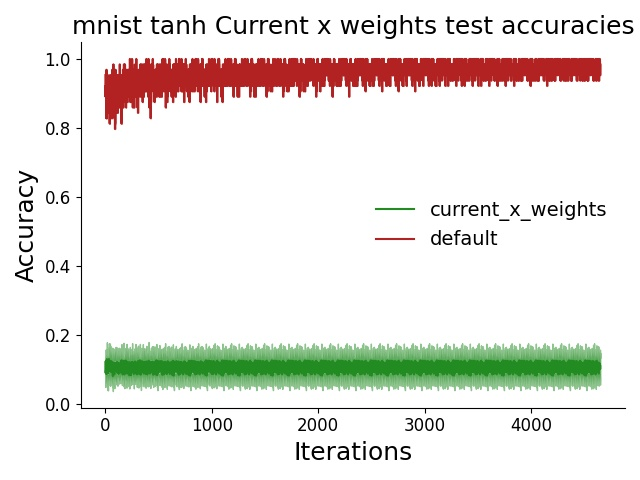
\includegraphics[width=0.75\linewidth]{chapter_6_figures/AR/mnist_tanh_Current_x_weights_test_accuracies_prelim_2.jpg} 
    \caption{MNIST current x weight update} 
  \end{subfigure} 
  \caption{Assessing whether the frozen feedforward pass assumption can be relaxed. We show the resulting performance (test accuracy) against baseline of relaxing this assumption on the MNIST dataset. See Appendix B for the Fashion-MNIST results. All results averaged over 10 seeds.}
  \label{AR_no_frozen_pass}
\end{figure} 

In Figure \ref{AR_no_frozen_pass}, we see that the frozen feedforward pass assumption can be relaxed in the case of the nonlinear derivatives for both the AR update and the weight update equation. However, relaxing it in the case of the weight update equation destroys performance. This means that ultimately, a direct implementation of AR in biological circuitry would require neurons to store the feedforward pass value of their own activations. 

All the experiments so far have been done on the relatively simple and straightforward MNIST dataset with small MLP models. However, it is also important to verify the scalability of this method. Here we demonstrate that AR can be used to train large CNNs on challenging image recognition datasets (SVHN, CIFAR10, and CIFAR100) and, moreover, that the previous loosenings of the biologically implausible constraints on the algorithm still do not appear to degrade performance unduly. This extension to CNNs is especially important because other biologically plausible schemes such as feedback alignment \citep{lillicrap2016random,lillicrap2014random}, and directed feedback alignment \citep{nokland2016direct}, have been shown to struggle with the CNN116architectures \citep{launay2019principled}. We tested the simplifications (dropping nonlinearity or learning backwards weights) on just the convolutional layers of the network, just the fully-connected layers of the network, or both together. We found that ultimately performance was largely maintained even when both convolutional and fully connected layers in the network used learnable backwards weights or had their nonlinear derivatives dropped from both the update and weight equations. These results speak to the scalability and generalisability of these relaxations, and the general robustness of the AR algorithm. We implemented the learnable backwards weights of the CNN by applying Equation \ref{BP_weights_equation} to the flattened form of the CNN filter kernel weights.

Our CNN consisted of a convolutional layer followed by a max-pooling layer, followed by an additional convolutional layers, then two fully connected layers. The convolutional layers had 32 and 64 filters respectively, while the FC layers had 64,120, and 10 neurons respectively. For CIFAR100 there are 100 output classes so the final layer had 100 neurons. The labels were one-hot-encoded and fed to the network. All input images were normalized so that their pixel values lay in the range $[0,1]$ but no other preprocessing was undertaken. We used hyperbolic tangent activations functions at every layer except the final layer which was linear. The network was trained on a mean-square-error loss function. 

 \begin{figure}[htb]
    \centering % <-- added
\begin{subfigure}{0.25\textwidth}
  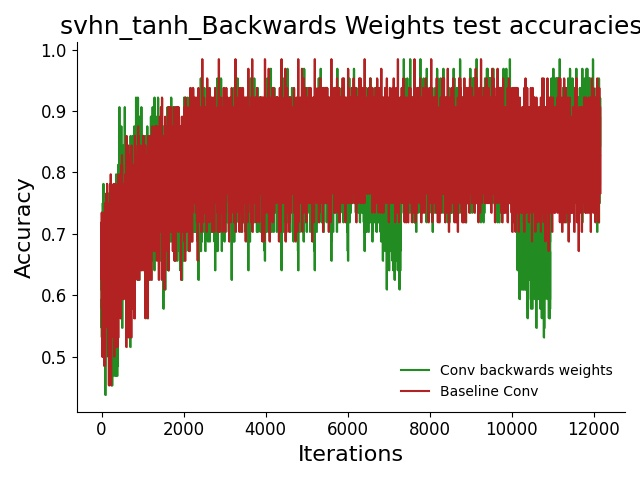
\includegraphics[width=\linewidth]{chapter_6_figures/AR/svhn_tanh_Backwards_Weights_test_accuracies_prelim_1.jpg}
  \caption{Conv backwards weights}
\end{subfigure}\hfil % <-- added
\begin{subfigure}{0.25\textwidth}
  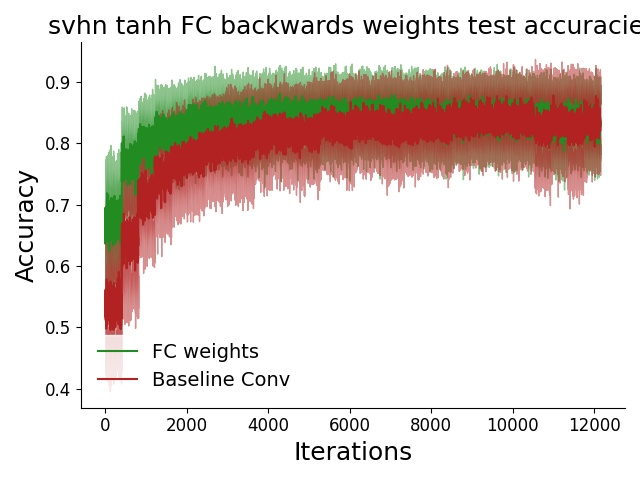
\includegraphics[width=\linewidth]{chapter_6_figures/AR/svhn_tanh_FC_backwards_weights_test_accuracies_prelim_1.jpg}
  \caption{FC backwards weights}
\end{subfigure}\hfil % <-- added
\begin{subfigure}{0.25\textwidth}
  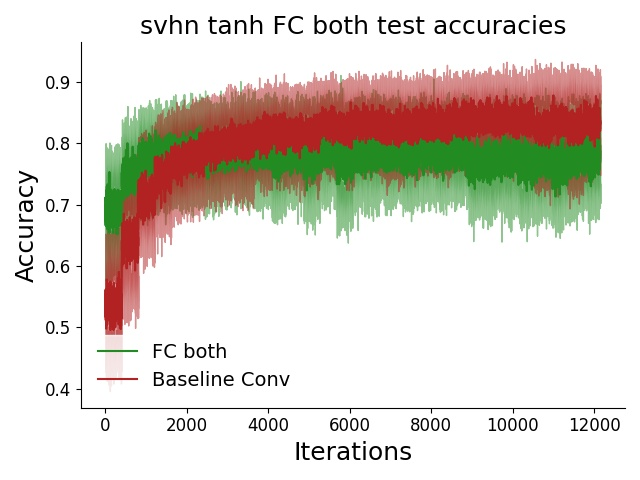
\includegraphics[width=\linewidth]{chapter_6_figures/AR/svhn_tanh_FC_both_test_accuracies_prelim_1.jpg}
  \caption{Both backwards weights}
\end{subfigure}

\medskip
\begin{subfigure}{0.25\textwidth}
  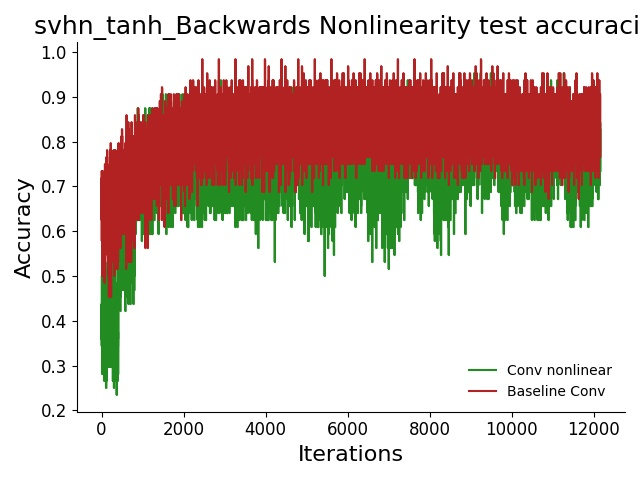
\includegraphics[width=\linewidth]{chapter_6_figures/AR/svhn_tanh_Backwards_Nonlinearity_test_accuracies_prelim_1.jpg}
  \caption{Conv no nonlinear derivative}
\end{subfigure}\hfil % <-- added
\begin{subfigure}{0.25\textwidth}
  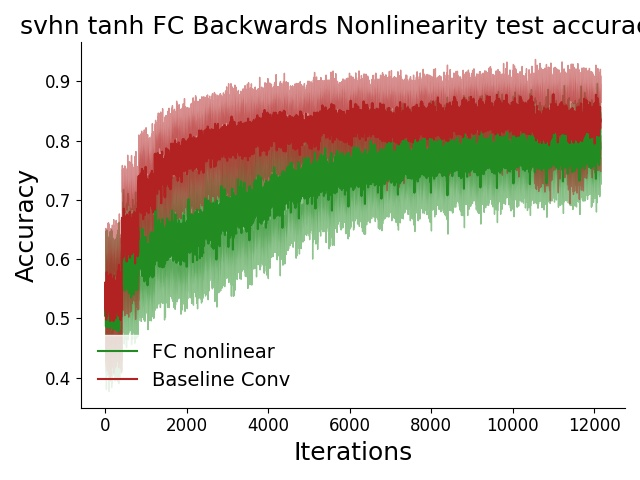
\includegraphics[width=\linewidth]{chapter_6_figures/AR/svhn_tanh_FC_Backwards_Nonlinearity_test_accuracies_prelim_1.jpg}
  \caption{FC no nonlinear derivative}
\end{subfigure}\hfil % <-- added
\begin{subfigure}{0.25\textwidth}
  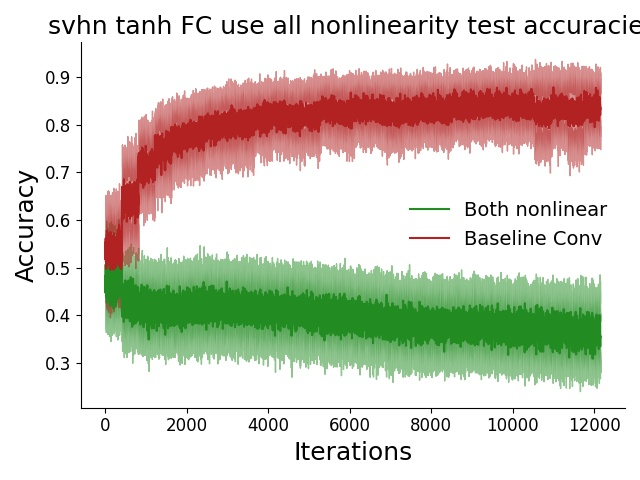
\includegraphics[width=\linewidth]{chapter_6_figures/AR/svhn_tanh_FC_use_all_nonlinearity_test_accuracies_prelim_1.jpg}
  \caption{Both no nonlinear derivative}
\end{subfigure}
%\caption{}
\end{figure}

We see that the simplifications also scale to the CNN for the SVHN dataset, although, interestingly, performance is degraded on this dataset when both convolutional and FC nonlinearities are dropped. However, since this does not occur in the other, more challenging, CIFAR datasets, we take this result to be an anomaly.


 \begin{figure}[htb]
    \centering % <-- added
\begin{subfigure}{0.3\textwidth}
  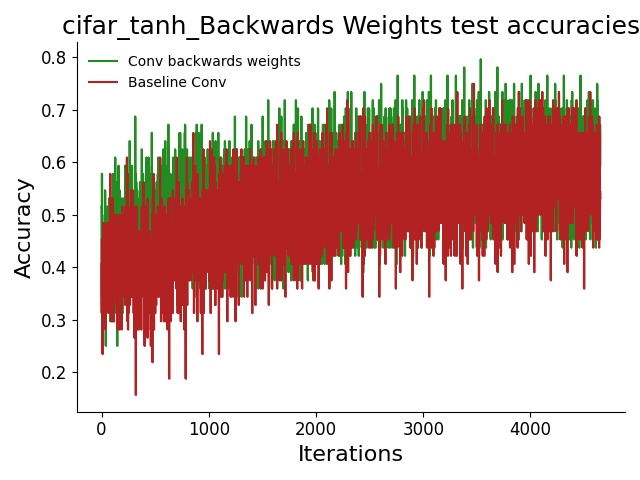
\includegraphics[width=\linewidth]{chapter_6_figures/AR/cifar_tanh_Backwards_Weights_test_accuracies_prelim_1.jpg}
  \caption{Conv backwards weights}
\end{subfigure}\hfil % <-- added
\begin{subfigure}{0.3\textwidth}
  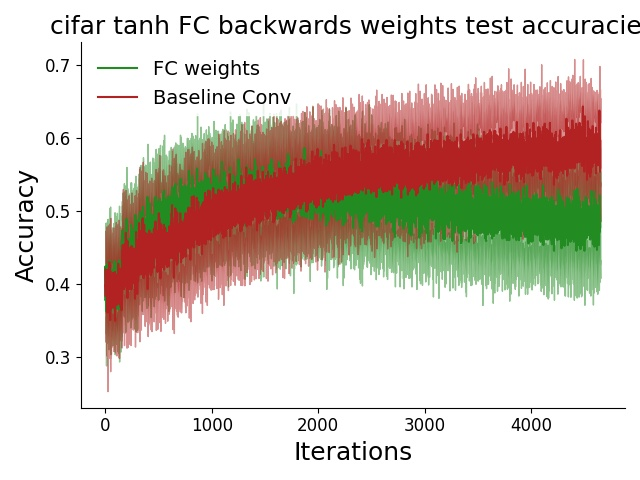
\includegraphics[width=\linewidth]{chapter_6_figures/AR/cifar_tanh_FC_backwards_weights_test_accuracies_prelim_1.jpg}
  \caption{FC backwards weights}
\end{subfigure}\hfil % <-- added
\begin{subfigure}{0.3\textwidth}
  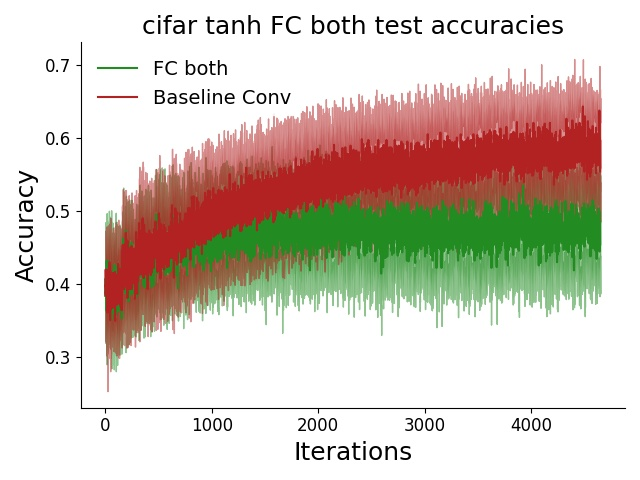
\includegraphics[width=\linewidth]{chapter_6_figures/AR/cifar_tanh_FC_both_test_accuracies_prelim_1.jpg}
  \caption{Both backwards weights}
\end{subfigure}

\medskip
\begin{subfigure}{0.3\textwidth}
  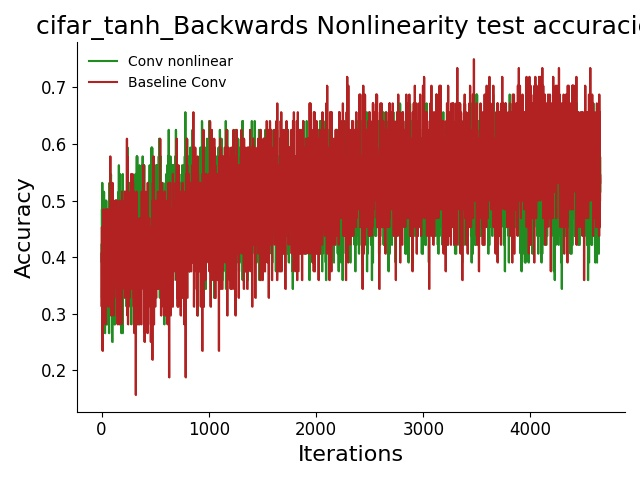
\includegraphics[width=\linewidth]{chapter_6_figures/AR/cifar_tanh_Backwards_Nonlinearity_test_accuracies_prelim_1.jpg}
  \caption{Conv no nonlinear derivative}
\end{subfigure}\hfil % <-- added
\begin{subfigure}{0.3\textwidth}
  \includegraphics[width=\linewidth]{chapter_6_figures/AR/cifar_tanh_FC_Backwards_Nonlinearity_test_accuracies_prelim_1.jpg}
  \caption{FC no nonlinear derivative}
\end{subfigure}\hfil % <-- added
\begin{subfigure}{0.3\textwidth}
  \includegraphics[width=\linewidth]{chapter_6_figures/AR/cifar_tanh_FC_use_all_nonlinearity_test_accuracies_prelim_1.jpg}
  \caption{Both no nonlinear derivative}
\end{subfigure}
\caption{Performance (test accuracy), averaged over 10 seeds, on CIFAR10 demonstrating the scalability of the learnable backwards weights and dropping the nonlinear derivatives in a CNN architecture, compared to baseline AR without simplifications. Performance is equivalent throughout.}
\end{figure}


 \begin{figure}[htb]
    \centering % <-- added
\begin{subfigure}{0.25\textwidth}
  \includegraphics[width=\linewidth]{chapter_6_figures/AR/cifar100_tanh_Backwards_Weights_test_accuracies_prelim_1.jpg}
  \caption{Conv backwards weights}
\end{subfigure}\hfil % <-- added
\begin{subfigure}{0.25\textwidth}
  \includegraphics[width=\linewidth]{chapter_6_figures/AR/cifar100_tanh_FC_backwards_weights_test_accuracies_prelim_1.jpg}
  \caption{FC backwards weights}
\end{subfigure}\hfil % <-- added
\begin{subfigure}{0.25\textwidth}
  \includegraphics[width=\linewidth]{chapter_6_figures/AR/cifar100_tanh_FC_both_test_accuracies_prelim_1.jpg}
  \caption{Both backwards weights}
\end{subfigure}

\medskip
\begin{subfigure}{0.25\textwidth}
  \includegraphics[width=\linewidth]{chapter_6_figures/AR/cifar100_tanh_Backwards_Nonlinearity_test_accuracies_prelim_1.jpg}
  \caption{Conv no nonlinear derivative}
\end{subfigure}\hfil % <-- added
\begin{subfigure}{0.25\textwidth}
  \includegraphics[width=\linewidth]{chapter_6_figures/AR/cifar100_tanh_FC_Backwards_Nonlinearity_test_accuracies_prelim_1.jpg}
  \caption{FC no nonlinear derivative}
\end{subfigure}\hfil % <-- added
\begin{subfigure}{0.25\textwidth}
  \includegraphics[width=\linewidth]{chapter_6_figures/AR/cifar100_tanh_FC_use_all_nonlinearity_test_accuracies_prelim_1.jpg}
  \caption{Both no nonlinear derivative}
\end{subfigure}
%\caption{}
\end{figure}


\subsection{Interim Discussion}

In sum the AR algorithm uses only simple learning rules to asymptotically approximate the adjoint terms of backprop over the course of multiple dynamical iterations. We have demonstrated that the AR algorithm can apply to arbitrary computation graphs, as can predictive coding, and can be used to train deep CNN models on challenging object recognition tasks with a performance equivalent to backprop. Moreover, AR eschews much of the complexity of competing schemes such as predictive coding, by not requiring two separate population of value and error neurons, and equilibrium propagation by not needing two separate backwards phases -- a free phase and a clamped phase. Additionally, we have demonstrated that some of the remaining biological implausibilities of AR, such as the weight transport and backwards nonlinearities problems, can be successfully ameliorated through the right extensions to the algorithm such as learnable backwards weights with minimal effect on overall performance. Other constraints, such as the necessity to use the feedforward pass activities in the dynamics instead of the current activities cannot be relaxed with catastrophically damaging overall performance.

Like predictive coding, a limitation of this method is its intrinsically iterative nature. This iteration scheme means that it is at least several times more costly than standard backpropagation of error -- for instance, in these experiments we used 100 iterations to reach exact convergence to the backpropagated gradients, although this is not strictly necessary for good performance. While some of this computational cost may be ameliorated by the intrinsic parallelism of neural circuitry, there is nevertheless a timing issue if convergence is required to be complete before the next sensory datum arrives, and issues of gradient interference if it is not. A speculative solution to this could be synchronization mediated by the brain's alpha/beta or gamma band frequencies in the cortex, where one dynamical phase iterating to convergence would correspond to one wavelength of the band. Such an identification is highly speculative however, and the computational function of such oscillations in the brain are still largely mysterious and highly controversial \citep{buzsaki2006rhythms}.

One additional and important drawback of the AR algorithm is that it requires keeping a memory of the feedforward pass activations throughout the backwards dynamical phase. This is because the activations swap their purpose from representing feedforward pass values in the forward phase, to representing gradients in the backwards phase. Taken literally, this requires that the learning rules become non-local in time, although in practice the feedforward pass activations are just stored. While this the most substantial drawback to the biological plausibility of the algorithm, it is important to note that this drawback is also shared with every other iterative algorithm in the literature. Predictive coding similarly requires the fixed-prediction assumption, which is effectively the same, and equilibrium-propagation requires that all the activations at the equilibrium of the free phase are stored while the clamped phase converges. We suggest that this necessity for storage in iterative algorithms to approximate backprop is universal and it arises for a simple reason. Namely, that the backpropagated gradients themselves fundamentally only depend upon the feedforward pass values, since we are backpropagating only on the feedforward pass and not through the dynamics themselves. Since the gradients ultimately depend only on the feedforward pass, any dynamical scheme to approximate them must `remember' what these values are, somehow. In theory, it may be possible to design algorithms such that this memory is implicit and thus not explicitly necessary, but no such algorithms have, to my knowledge, been found so far.

This issue of memory is also closely related to the core computational properties of reverse-mode AD. Specifically, that it requires storage in memory of all intermediate activations in the forward pass. This means that the memory issue also closely applies to sequential backward algorithms such as target-propagation and, indeed, backprop itself. The fundamental fact is that backwards pass can only take place \emph{after} the forward pass is complete, and that it requires knowledge of forward pass activities. This fact cannot be ignored or cleverly wished away by any algorithm but must simply be addressed. If the brain is performing reverse-mode AD, then it simply must have some way to store, implicitly or explicitly, the feedforward pass values. The question then becomes how can this be done in the brain? Some possibilities are multiplexing using the brain's own intrinsic rhythms \citep{buzsaki2006rhythms}, or some kind of special parallel class or neurons to maintain activity explicitly \citep{o1999biologically}, or else storage at the synaptic level through mechanisms like eligibility traces \citep{bellec2020solution}. While we here remain ambiguous on the means by which such storage is achieved, we have reached a point of conceptual clarity in knowing that there \emph{must be storage}. The only question is how.
% I'll discuss the general issues with the fixed prediction assumptions etc here

\section{Three-Factor Learning Rules and a Direct Implementation}

After having gone through several iterative algorithms for approximating the backpropagation of error algorithm, it is worth taking a step back to understand what has been shown and what is truly necessary. Here, we argue that in fact, despite strong claims that backprop is biologically implausible, in fact an actual implementation of backprop in the brain could be surprisingly simple and biologically plausible. Moreover, that many of the algorithms, including the iterative algorithms previously, may simply be complicating matters. The material in this section is speculative and early stage, and will be investigated further in future work.

First, we begin by stating, somewhat boldly, that in general the weight transport problem is solved. That is, there is now fairly strong evidence in the literature \citep{lillicrap2016random,amit2019deep,akrout2019deep,millidge2020relaxing} firstly that a precise equality of forward and backwards weights is not necessary for good learning performance, and secondly, that competitive performance with backprop can be maintained, even for deep networks, through learnable backwards weights which update with a fairly straightforward Hebbian learning rule. If we assume that the weight transport problem is solved, then there is only the locality issues remaining with a direct implementation of backprop.

Firstly, we note that if we are implementing reverse-mode AD, and we find a way to compute the adjoint $\frac{\partial \mathcal{L}}{\partial x^l}$ locally at a layer then we actual weight update $\frac{\partial \mathcal{L}}{\partial W^l} = \frac{\partial \mathcal{L}}{\partial x^l}\frac{\partial x^l}{\partial W^l}$ requires only local information. This means that almost the entire challenge of backprop is computing the adjoint term locally.

Secondly, we notice that the standard forward pass of an artificial neural network $x^l = f(W^l x^{l-1})$ does not actually correspond to how it would work in the brain since here the activation function (which is typically assumed to be applied through the threshold for making an action potential in the cell soma) is applied \emph{after} the weights, while in the brain the synaptic weights are on the dendrites of the post-synaptic neuron, and thus occur after the action potential. This means that instead we should use the more biologically plausible forward pass as,
\begin{align*}
\label{forward_equation}
    x^l = W^l f(x^{l-1}) \numberthis
\end{align*}
Where the order of the weights and the activation function are switched. Specifically, this means that the activation function only applies to the presynaptic activity and not the weights. This approach considerably simplifies the requisite gradients, so we get the following expressions for the adjoint and the weight update
\begin{align*}
    \frac{\partial \mathcal{L}}{\partial x^l} &=\frac{\partial \mathcal{L}}{\partial x^{l+1}} {W^{l+1}}^T f'(x^l) \\
    \frac{\partial x^l}{\partial W^l} &=  \frac{\partial \mathcal{L}}{\partial x^l} f(x^l) \numberthis
\end{align*}

Specifically, the adjoint recursion is simply the adjoint of the layer above, multiplied through the backwards weights and the derivative of the activation function of the pre-synaptic activity. The weight update is substantially simpler since, because the forward pass is linear in the weights, it is simply a multiplication of the adjoint with the presynaptic activity which is essentially Hebbian except with the adjoint replacing the post-synaptic term. Interestingly, this applies that in this case of backprop, the post-synaptic term should have \emph{no} effect on the synaptic weights, which is a very strong and counterintuitive empirical prediction of backprop. 

While it may seem that the switch in the order of the weights and the activation function might have some serious impact on the expressive power of the network, we argue that it likely does not. In fact, the two formulations are equivalent in deep neural networks except for the beginning and ending layers. To see this, we can simply explicitly write out the expression for the function computed by 4 layer neural network,
\begin{align*}
    y = f(W^4 f(W^3 f(W^2 f(W^1 x)))) \approx W^4 f(W^3 f(W^2 f(W^1 f(x)))) \numberthis
\end{align*}
For the vast majority of layers, these expressions are the same up to a re-bracketing. The only difference is the last layer has no activation function using the more neural forward pass (but often in neural networks we use a linear last layer anyway), and that the input is first passed to an activation function activation function where this is not common in standard ANNs -- but this function could always be set to the identity to make the equivalence exact. In general, the effect of these differences will be minor for deep networks.

Now we note the crucial point, that the only biological implausibilities in these learning rules is the necessity to have the adjoint value present at the synapse for the weight update rule, since it is just the multiplication of the adjoint and the presynaptic activation. The recursive computation of the adjoint itself (Equation \ref{reverse_mode_equation} is relatively plausible, since the only difficulty is the nonlinear derivative term $f'(x)$ which now is only the derivative of the activation function applied to the pre-synaptic input. Importantly, for spiking neurons, this derivative is trivial as is essentially consists of a spike when the neuron fires and not when it doesn't. As such, this rule effectively says that the adjoint should only be updated when there is presynaptic firing. Putting this all together, we can imagine implementing this in the brain in a fairly direct forward-backward scheme as in Figure \ref{continuous_bp_figure}

\begin{figure}
    \centering
    \includegraphics[width=\linewidth]{chapter_6_figures/continuous_backprop_idea_v2.pdf}
    \caption{Potential schematic for a direct implementation of backprop in the brain. All that is necessary for this to be plausible is three-factor learning rules.}
\label{continuous_bp_figure}
\end{figure}

Specifically, if we assume that the weight transport problem can be solved with independently learnable backwards weights, then the recursion for the adjoint becomes simply,
\begin{align*}
    \frac{\partial \mathcal{L}}{\partial x^l} &=\frac{\partial \mathcal{L}}{\partial x^{l+1}} \psi^T f'(x^l) \\
    &\approx \frac{\partial \mathcal{L}}{\partial x^{l+1}} \psi^T \numberthis
\end{align*}
where the second line is the recursion if we simply ignore the nonlinear derivative term, as we have also found does not hinder learning in practice \citep{millidge2020relaxing,millidge2020investigating,millidge2020activation,ororbia2019biologically}. This recursion is extremely simple and is just the adjoint mapped through the backwards weights to the layer below. Thus, we can imagine keeping separate forward and backward passes whereby the adjoint is represented by interneurons $I^l$. Here, the update rules simply become,
\begin{align*}
\label{continous_bp_backward_equation}
       I^l &=I^{l+1}\psi ^T  \\
    \frac{\partial \mathcal{L}}{\partial W^l} &=  I^l f(x^l) \numberthis
\end{align*}

The simplicity of these update rules imply show that the only potential biological implausibility is in the weight update \ref{BP_weights_equation} where we have transmitted the value of the adjoint `interneurons' to the synapses of the post-synaptic neuron, and used them to update those weights. Through a careful analysis, we have revealed this question to be the ultimate crux of whether backprop in the brain is plausible or not. Importantly, this ability to use the adjoints as part of a `local' learning rule is crucial to every purported `biologically-plausible' method in the literature -- from predictive coding, to target-propagation, to equilibrium-prop and AR. 

Whether or not the adjoint can be transmitted to the synaptic weights in the brain is currently a controversial and unresolved question, and to my knowledge, has not been studied directly. While it may seem fairly obscure, this analysis suggests that this question is absolutely crucial to our understanding of whether the brain can directly implement backprop or not. An important possibility is that of segregated dendrites \citep{sacramento2018dendritic}. Having separate dendritic compartments would, presumably, straightforwardly enable the broadcast of the adjoint values to the synaptic weights, since they would be located in the dendritic tree of the same neuron. The key question would then become whether information transmitted to the dendrites could remain segregated. That is, could both Equation \ref{forward_equation} and Equation \ref{continous_bp_backward_equation} be implemented using the same neuron. If this is the case then it would suggest an incredibly simple biological implementation for backpropagation, needing only a single type of neuron which would both send forward connections and reciprocally receive backwards connections from neurons in the layer above. Such a simple architecture would lend great support to the idea that the brain can indeed implement backprop, and perhaps that backpropagation is so straightforward that it may even function as a computational primitive in neural circuitry.

\section{Discussion}

Overall, in this chapter, we have shown that predictive coding, as an approximation to the backpropagation of error algorithm, can be extended to arbitrary computation graphs and we have applied predictive coding to large-scale machine learning architectures such as CNNs and LSTMs and demonstrated that they perform comparably to backprop trained networks. Moreover, we have posited a novel iterative algorithm -- Activation Relaxation -- that also converges to the exact backprop gradients, does not require two separate populations of predictions and prediction error units, and uses extremely simple and elegant learning and update rules. We have shown that AR also scales to large-scale CNN neural network models and is competitive with backprop trained networks at scale. Finally, taking experience from our previous work in this field, we have re-analyzesd the problem of backpropagation in the brain from first principles and discovered, somewhat surprisingly, that if we assume that the weight transport problem is solved, the only major issue of biological implausibility is whether recursively computed adjoints can be `transferred' onto synapses to be able to form part of the synaptic weight updates. If they can, and it seems likely that this is possible through a mechanism of segregated dendrites or, alternatively, backpropagating action potentials \citep{stuart1997action}, then we can be fairly certain that backproapgation in the brain is at least theoretically achievable. This is a remarkable turn-around from the consensus only five years ago that it was completely biologically implausible, and speaks to the rapid development and advances in this field.

Additionally, while this thesis chapters has presented an substantial extension to an existing algorithm (predictive coding), and an entirely novel algorithm for credit assignment in the brain (activation relaxation), we also wish to highlight the conceptual contributions we have made while thinking about these issues deeply. In my opinion, these are perhaps the most important sections of this work. Namely, firstly, the issue of memory and time in any implementation or approximation to reverse-mode AD. Specifically, that any biologically plausible algorithm, whether sequential or iterative, due to the very nature of reverse-mode AD \emph{must} store the values of the feedforward pass throughout the backwards sweep or phase, either implicitly or explicitly. While the rationale for this seems obvious in retrospect, it was not clear beforehand, and is still not at all clear in the literature. Indeed, the dependence of almost all of these biologically plausible algorithms on the memory of forward pass values is generally obfuscated or presented as a minor hindrance, when in fact it is an absolutely irrevocable fact of the comptuation these algorithms are trying to render biologically plausible. Secondly, and perhaps most importantly, we have reached the crux of the issue of whether backpropagation in the brain is plausible -- namely whether adjoints, which must remain separate from the post-synaptic activation -- can modulate synaptic weight updates. If they can, then very biologically plausible and elegant schemes exist for a direct implementation of backpropagation in the brain (see Equations \ref{continous_bp_backward_equation}, \ref{BP_weights_equation}). If it is not possible, then it seems likely, given that the adjoint equation is absolutely fundamental to reverse-mode AD, that backpropagation in the brain is not plausible or, at least, is explicitly achievable except via some roundabout method. Moreover, if the transport of the adjoint onto the synaptic weight terminals is possible, then it must be supported by some kind of dedicated neurophysiological mechanism, which can and must be studied in detail if we are to understand the explicit details of this key aspect of credit assignment in the brain. Nevertheless, I now believe that the key mathematical and conceptual issues in the question of whether the brain can do backpropagation (in this rate-coded static model) have been largely worked out and depend now solely on details of neurophysiology.

The crucial caveat to this response is that we have only worked out credit assignment in an incredibly simplified model of what occurs in the brain -- namely with rate-coded integrate and fire neurons -- on static inputs. Both of these assumptions, however, are false in the brain. Firstly, neurons are spiking networks which may communicate using precise spike timings to convey information. Understanding how to perform credit assignment in such spiking networks is still a young and open field, although there has been much recent progress \citep{schiess2016somato,zenke2018superspike,kaiser2020synaptic,neftci2019surrogate}. Moreover, and crucially, the key problem the brain faces is not just backpropagation through space (i.e. layers), but backpropagation through time. The brain must be able to assign credit correctly to temporally distant events from the synaptic weight values that, ultimately caused them. While a mathematical formulation of reverse-mode AD can be directly formulated by simply performing backprop on a computation graph `unrolled through time', in practice this means that in the backwards phase that \emph{time must run backwards} or, alternatively that the network must store not only the feedforward pass, but its \emph{entire history}, which is definitely biologically implausible. The key question is thus how to implement backpropagation through time in a biologically plausible manner. There has been much recent progress in this field, also combined with spiking networks such as \citep{zenke2018superspike,bellec2020solution}. However, the innovative approach engendered by E-prop only applies to single layer recurrent networks, leaving open the question of how to marry backpropagation through space and backpropagation through time.

An additional interesting consideration is that throughout, and generally in the literature, only reverse-mode AD is considered to be a contender for the credit assignment algorithm implemented in the brain. This is due to the historical use and generally better computational properties of reverse-mode for artificial neural networks \citep{griewank1989automatic,baydin2017automatic} and has thus become the dominant paradigm \citep{goodfellow2016deep,rumelhart1985feature,silver2017mastering}. However, this is not necessarily the case in highly parallel architectures like the brain, for which additional forward computation cost may be effectively negligible due to the degree of parallelization. Forward-mode AD can be implemented through dual numbers -- which directly pair activations with their derivatives, and which it is interesting to think about how this could relate to neural activity and synapses. Moreover, a key computational advantage of forward-mode AD is that it imposes no memory cost, since it is entirely online and requires no storage of intermediate activations, thus entirely obviating the memory issues inherent in implementations of reverse-mode AD. The disadvantage, however, with forward-mode AD in the brain is that it dislocates the derivative computation from the physical location of the synapses. The computations and derivatives `move forwards' up through higher layers and levels of processing while the synapses remain firmly put. it is necessary, then, whenever the computations and derivatives reach the end of the process to transmit the fully computed derivatives back to where they originated. Precisely working out this process has, to my knowledge, not yet been done, but it may result in a practicable algorithm. One important case where forward-mode AD makes sense is in backpropagation through time since, as the computation moves forward in time, so do the synapses themselves. Thus, the correct derivatives are always locally available precisely when they are needed. Forward-mode AD through time is known as real-time-recurrent learning (RTRL) \citep{williams1989experimental}, and is potentially a good algorithm for the brain to solve recurrence, although it is extremely computationally expensive, rendering it uncompetitive with reverse-mode BPTT for training large neural networks. Moreover, by taking various sparse approximations to RTRL, it is possible to reduce the computational cost at the cost of somewhat reduced learning performance. Algorithms such as eligibility-prop essentially try to make RTRL updates biologically plausible, with some success.

\section{Conclusion}

In this chapter, we have proposed two novel biologically plausible algorithms for credit assignment in the brain. Firstly, we demonstrate that predictive coding, under the fixed prediction assumption, and setup in a `reverse mode' naturally computed the gradients required for the backpropagation of error algorithm, as its dynamics satisfy the same recursive structure of the adjoint equation and thus, the fixed points of the prediction errors, upon convergence, equal the backpropagated error gradients which can then be used to perform backprop. We have extensively empirically validated this correspondence and used it to train large-scale and complex machine learning architectures such as CNNs and LSTMs with performance equal to those trained by backprop. 

Secondly, we have utilized the insights gained by our work with predictive coding to derive a new, and much simpler algorithm which we call \emph{Activation Relaxation} (AR). Here, instead of using separate prediction error neurons, we simply update the activation of the value neurons themselves to become equal to the backpropagated errors during the backwards iteration phase. While this eschews the fixed feedforward pass assumption required for predictive coding, it introduces a similar requirement of storing the initial feedforward pass value throughout the backwards iteration phase, so that they can then be used during the weight updates. We also empirically validate this correspondence and demonstrate that AR can be used to train machine learning architectures with the same performance as backpropagation. Importantly, we also investigate the potential for applying the same biologically plausible relaxations to the AR algorithm as we applied to predictive coding in Chapter 3, and show that the relaxations perform just as well in this new setting -- speaking to robustness and generalizability of these relaxations. Overall, we believe the AR algorithm is simpler, more elegant, and more biologically plausible than competing iterative backprop schemes such as predictive coding and equilibrium-propagation. However, it suffers from the limitations inherent in all iterative approaches -- the necessity to somehow store the feedforward pass values throughout the backwards pass. A clear understanding of this limitation, then opens the way for future work to try to remedy it or propose a different method entirely for solving backpropagation in the brain.

Finally, we have included some current (and unpublished) speculations on the potential solution to backpropagation in the brain for simple feedforward networks of rate-coded integrate and fire neurons, and have constructed a relatively direct method of implementing backpropagation with only a few moving components. Importantly, this construction relies heavily first on its nonstandard definition of the forward pass, using $x^{l+1} = W f(x^l)$  -- or the weights after the activation function, rather than inside of it -- which is non-standard for artificial neural networks, but is actually more biologically plausible, and secondly on the solution to the weight transport problem to allow for learnable backward weights. With these issues circumvented, we believe that biologically plausible backpropagation for rate-coded integrate and fire neurons actually turns out to be relatively straightforward. The key next move for future work, now that this base of understanding is established, is to start to attack the substantially harder problem of biologically plausible implementations of backpropagation through time, as well as with spiking neuron models.

Overall, in this chapter, we believe that we have made several clear contributions towards understanding the biological plausibility of backpropagation in the brain -- firstly by providing and empirically validating two new iterative algorithms (predictive coding and activation relaxation) and secondly by coming to a much clearer understanding of what exactly the remaining stumbling blocks to a biological implementation are.